\mainmatter
\pagestyle{headings}
\chapter{Research}
\label{ch:research}

\section{Analysis}
The whole data set and data analysis script can be found on the GitHub repository\footnote{https://github.com/MoutPessemier/A-Survey-On-The-Impact-of-Customer-Chatbots-on-E-commerce}.\\
\break
The data has been anonymised in Excel. A new column was created called 'taskCategory'. The tasks performed are categorised in one of the following four categories:
\begin{itemize}
	\setlength\itemsep{-0.1em}
	\item FAQ
	\item Personalised question
	\item Complaint
	\item Sales
\end{itemize}
From the 65 entries, five had to be thrown away:
\begin{itemize}
	\setlength\itemsep{-0.1em}
	\item Three because of the used chatbot: they were not telecom chatbots.
	\item One entry was a duplicate.
	\item One entry responded with one answer only (only yes and only neutral in part 2)
\end{itemize}

\subsection{Environment Variables}
\subsubsection{Age}
The mean and standard deviation values for each provider respectively are:
\begin{itemize}
	\setlength\itemsep{-0.1em}
	\item \textbf{Overall: 26.28 \& 7.49}
	\item Telenet: 26.96 \& 9.73
	\item Proximus: 27.26 \& 6.07
	\item Orange: 22.5 \& 2.12
	\item T-Mobile: 22.44 \& 2.01
	\item KPN: 27.75 \& 3.59
\end{itemize}
Next to the plot, there is a frequency table that shows the different values for age appearing in this survey, ordered from most common to least common (Figure \ref{fig:agePlot} and \ref{fig:ageFreq}).

\begin{figure}[!htb]
	\minipage{0.75\textwidth}
	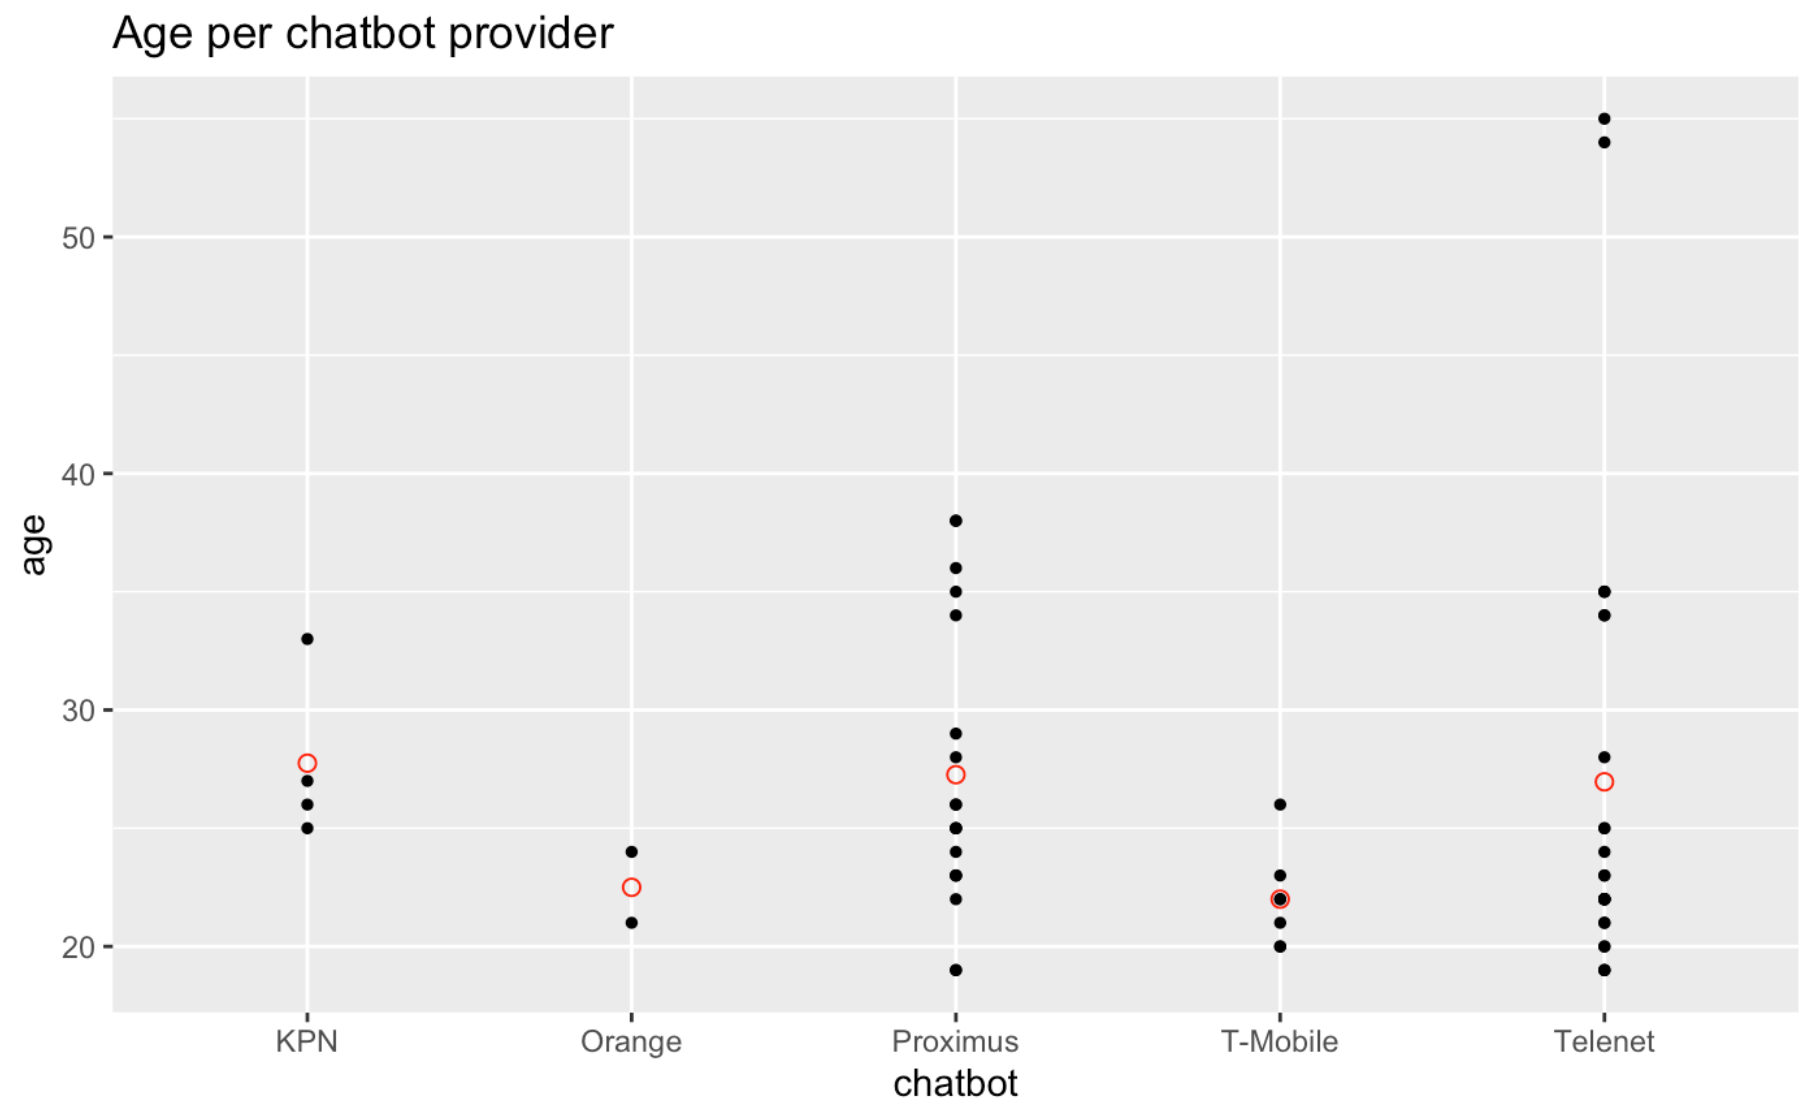
\includegraphics[width=\linewidth]{../LaTeX/Figures/Environments/AgePlot.png}
	\caption{The distribution of the age variable per chatbot provider.}\label{fig:agePlot}
	\endminipage\hfill
	\minipage{0.24\textwidth}
	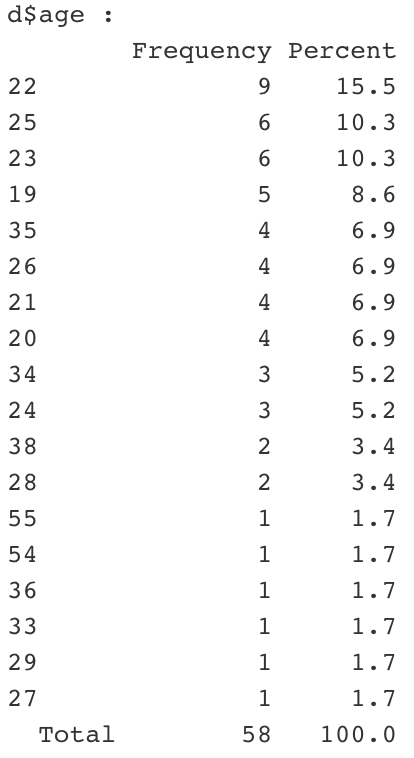
\includegraphics[width=\linewidth]{../LaTeX/Figures/Environments/AgeFreq.png}
	\caption{A frequency table of all the entries' ages.}\label{fig:ageFreq}
	\endminipage\hfill
\end{figure}


\subsubsection{Highest degree}
Looking at the acquired degrees of the respondents, the most common category is a master degree with 19 respondents, followed by an academic bachelor with 17 answers. Third comes high school with 12 (see Figure \ref{fig:degreePlot} and \ref{fig:degreeFreq}).
\begin{figure}[htb!]
	\minipage{0.55\textwidth}
	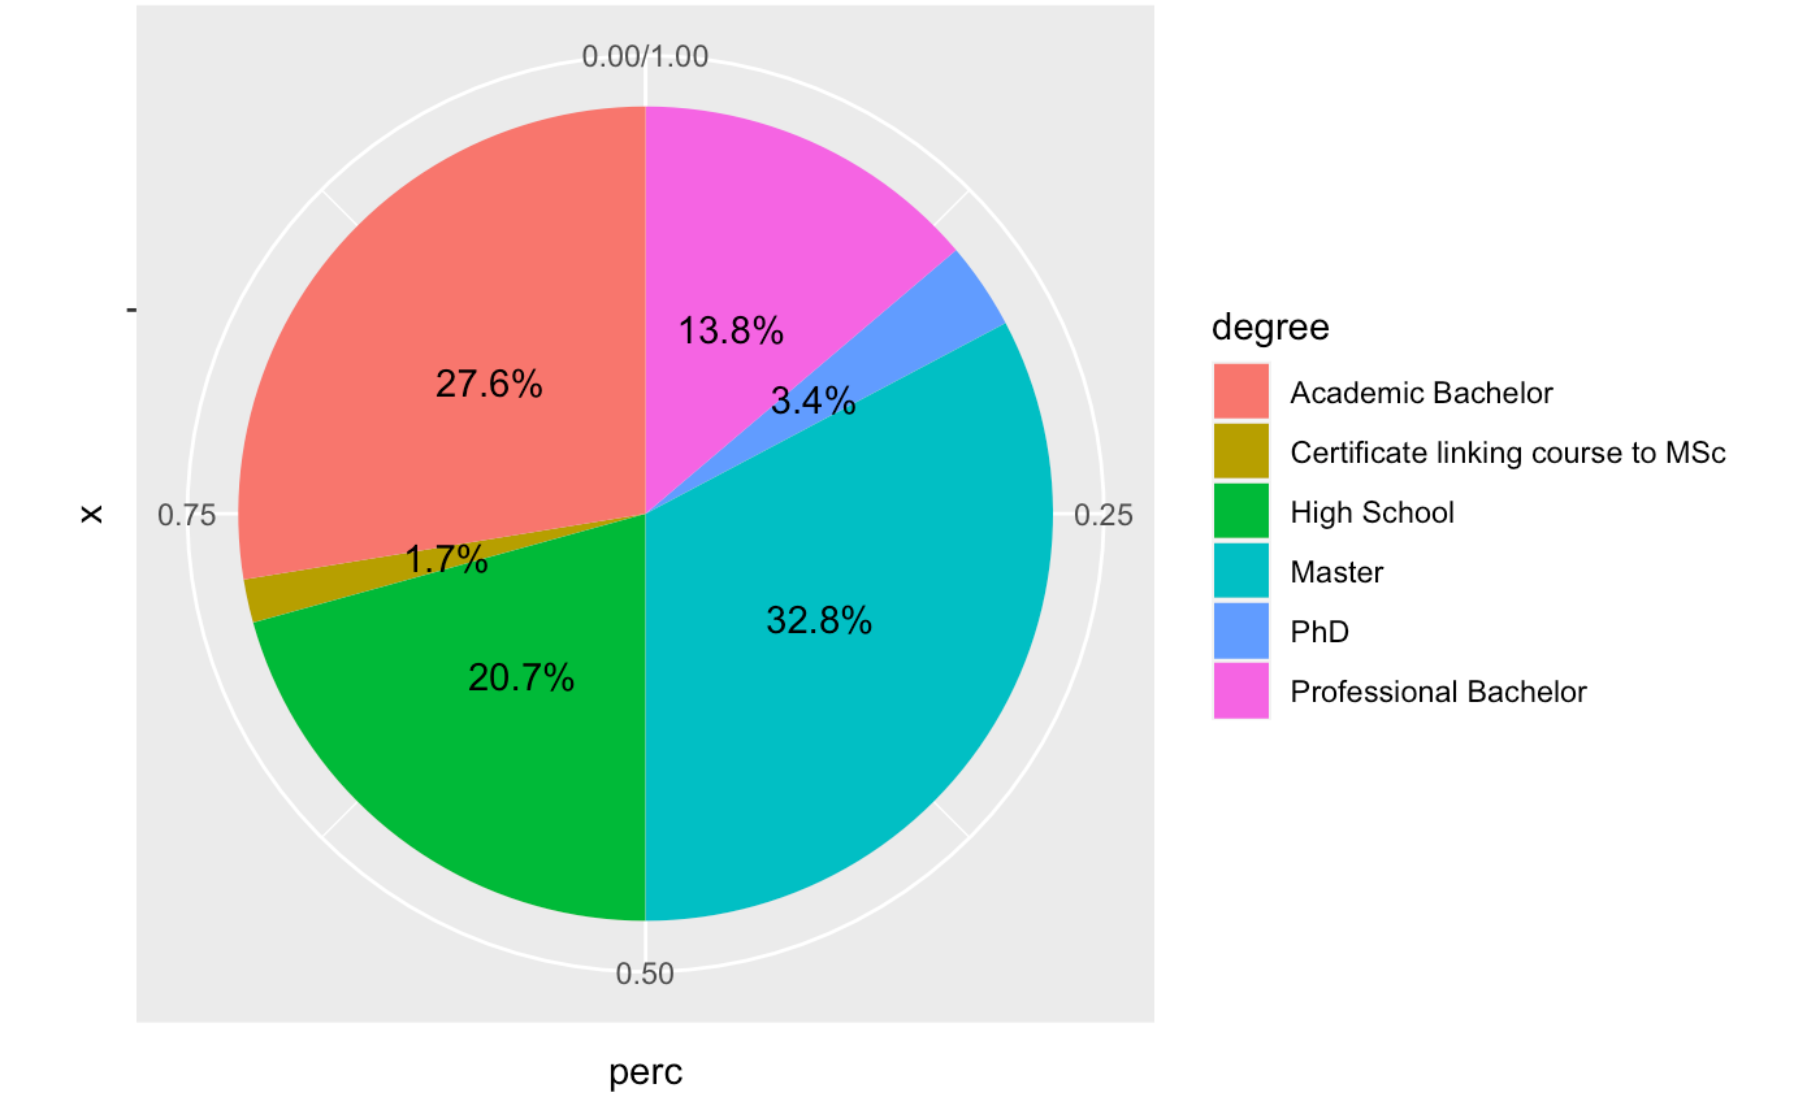
\includegraphics[width=\linewidth]{../LaTeX/Figures/Environments/DegreePlot.png}
	\caption{The distribution of the degree variable.}\label{fig:degreePlot}
	\endminipage\hfill
	\minipage{0.44\textwidth}
	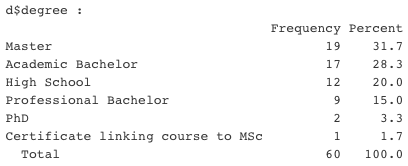
\includegraphics[width=\linewidth]{../LaTeX/Figures/Environments/DegreeFreq.png}
	\caption{A frequency table of all the entries' degrees.}\label{fig:degreeFreq}
	\endminipage\hfill
\end{figure}

\subsubsection{Gender}
There were 34 males who filled in the survey and 25 females. One person identified as non-binary (see Figure \ref{fig:genderPlot} and \ref{fig:genderFreq}).
\begin{figure}[!htb]
	\minipage{0.69\textwidth}
	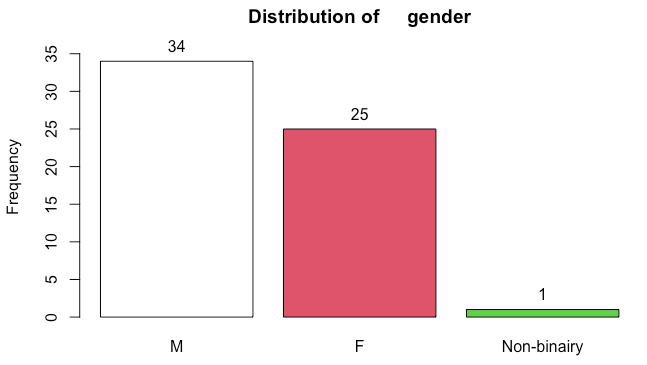
\includegraphics[width=\linewidth]{../LaTeX/Figures/Environments/GenderPlot.png}
	\caption{The distribution of the gender variable.}\label{fig:genderPlot}
	\endminipage\hfill
	\minipage{0.30\textwidth}
	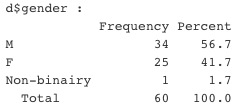
\includegraphics[width=\linewidth]{../LaTeX/Figures/Environments/GenderFreq.png}
	\caption{A frequency table of all the entries' genders.}\label{fig:genderFreq}
	\endminipage\hfill
\end{figure}

\subsubsection{Company of chatbot}
Telenet has the most respondents, followed by Proximus. The other chatbot providers are less represented (see Figure \ref{fig:chatbotPlot} and \ref{fig:chatbotFreq}).
\begin{figure}[!htb]
	\minipage{0.69\textwidth}
	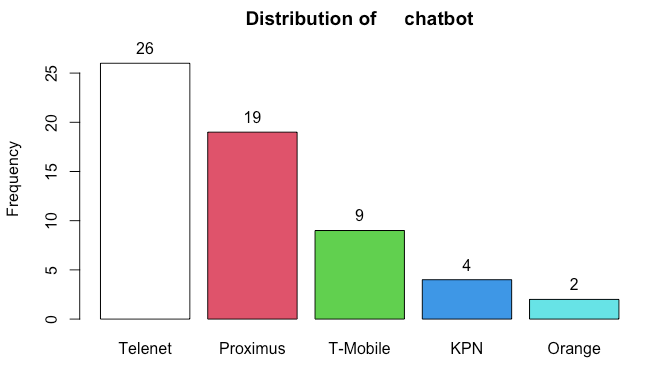
\includegraphics[width=\linewidth]{../LaTeX/Figures/Environments/ChatbotPlot.png}
	\caption{The distribution of the different chatbot providers and the amount of respondents for each provider.}\label{fig:chatbotPlot}
	\endminipage\hfill
	\minipage{0.30\textwidth}
	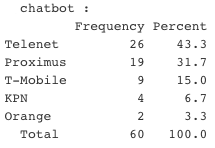
\includegraphics[width=\linewidth]{../LaTeX/Figures/Environments/ChatbotFreq.png}
	\caption{A frequency table of all the entries' used chatbots.}\label{fig:chatbotFreq}
	\endminipage\hfill
\end{figure}

\subsubsection{Used language}
Most users used Dutch as their preferred language of interaction which does not come as a surprise since this thesis focuses on the Flemish part of Belgium along with the Netherlands. Afterwards, English was the second most used language and French came last (see Figure \ref{fig:languagePlot} and \ref{fig:languageFreq}).

\begin{figure}[!htb]
	\minipage{0.69\textwidth}
	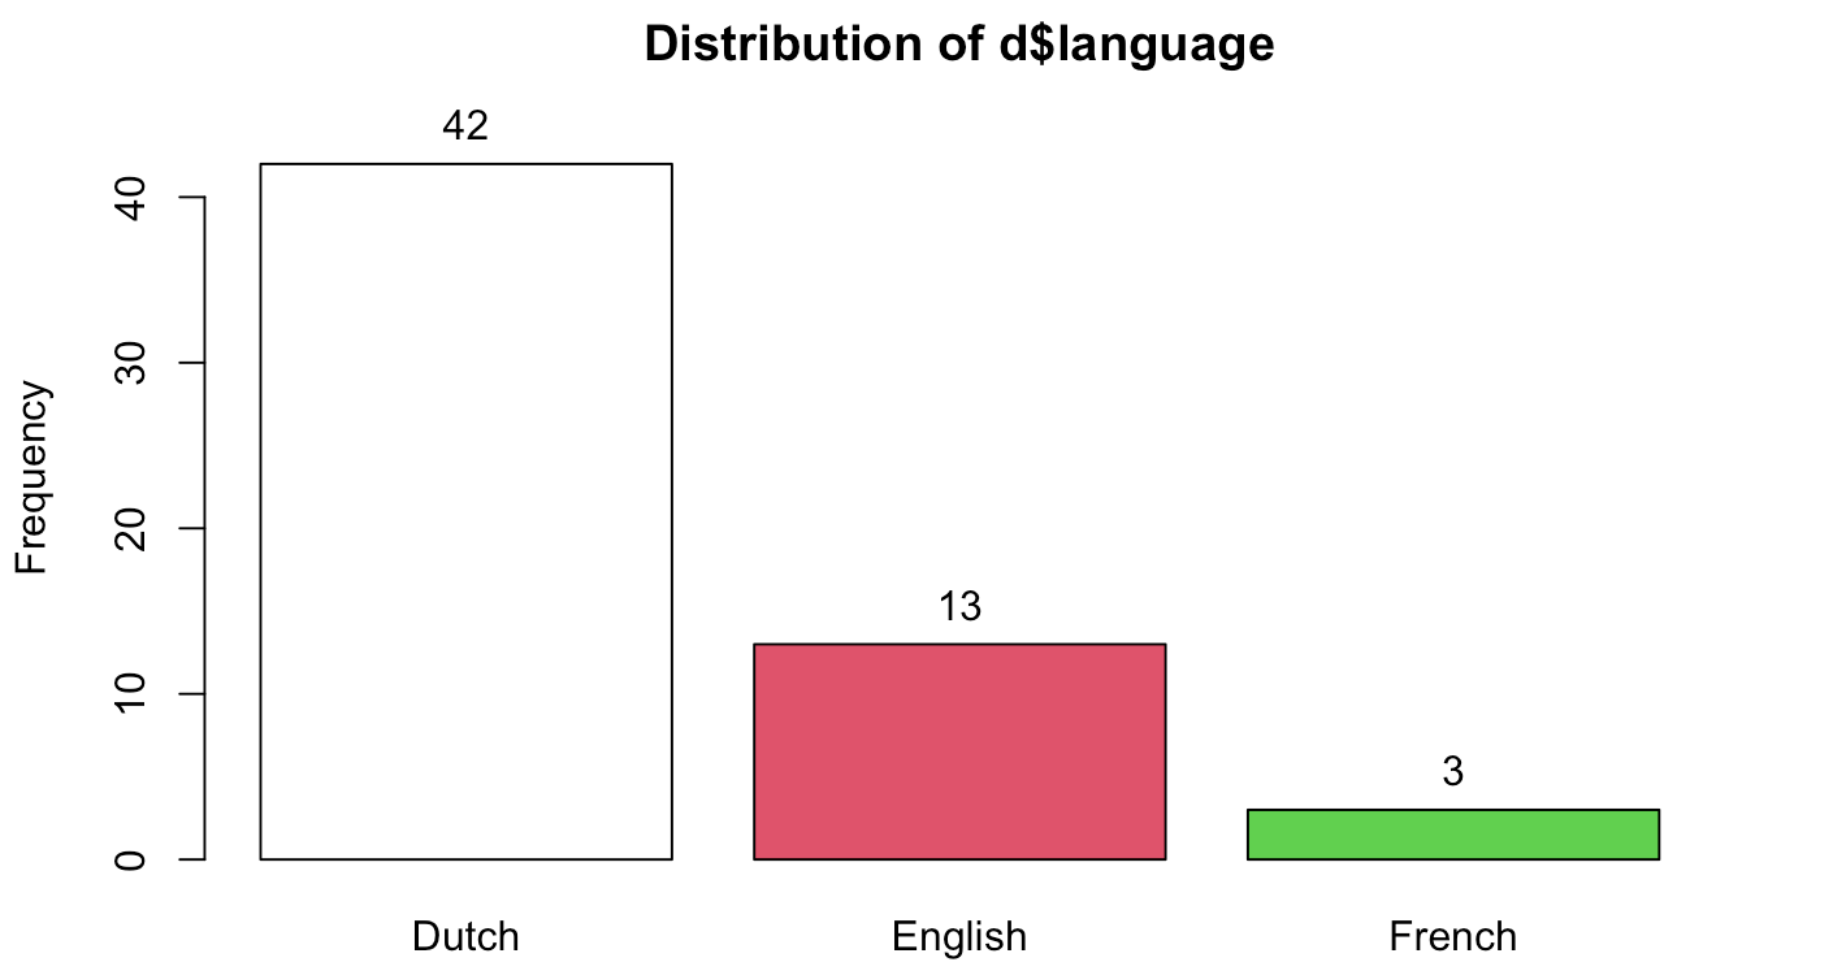
\includegraphics[width=\linewidth]{../LaTeX/Figures/Environments/LanguagePlot.png}
	\caption{The distribution of the language variable.}\label{fig:languagePlot}
	\endminipage\hfill
	\minipage{0.30\textwidth}
	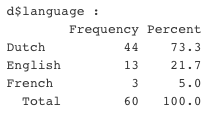
\includegraphics[width=\linewidth]{../LaTeX/Figures/Environments/LanguageFreq.png}
	\caption{A frequency table of all the entries' used languages.}\label{fig:languageFreq}
	\endminipage\hfill
\end{figure}

\subsubsection{Platform}
Most chatbots were used on the website of the provider themselves. Only a small percentage were used in app or via Facebook Messenger (see Figure \ref{fig:platformPlot} and \ref{fig:platformFreq}).

\begin{figure}[!htb]
	\minipage{0.69\textwidth}
	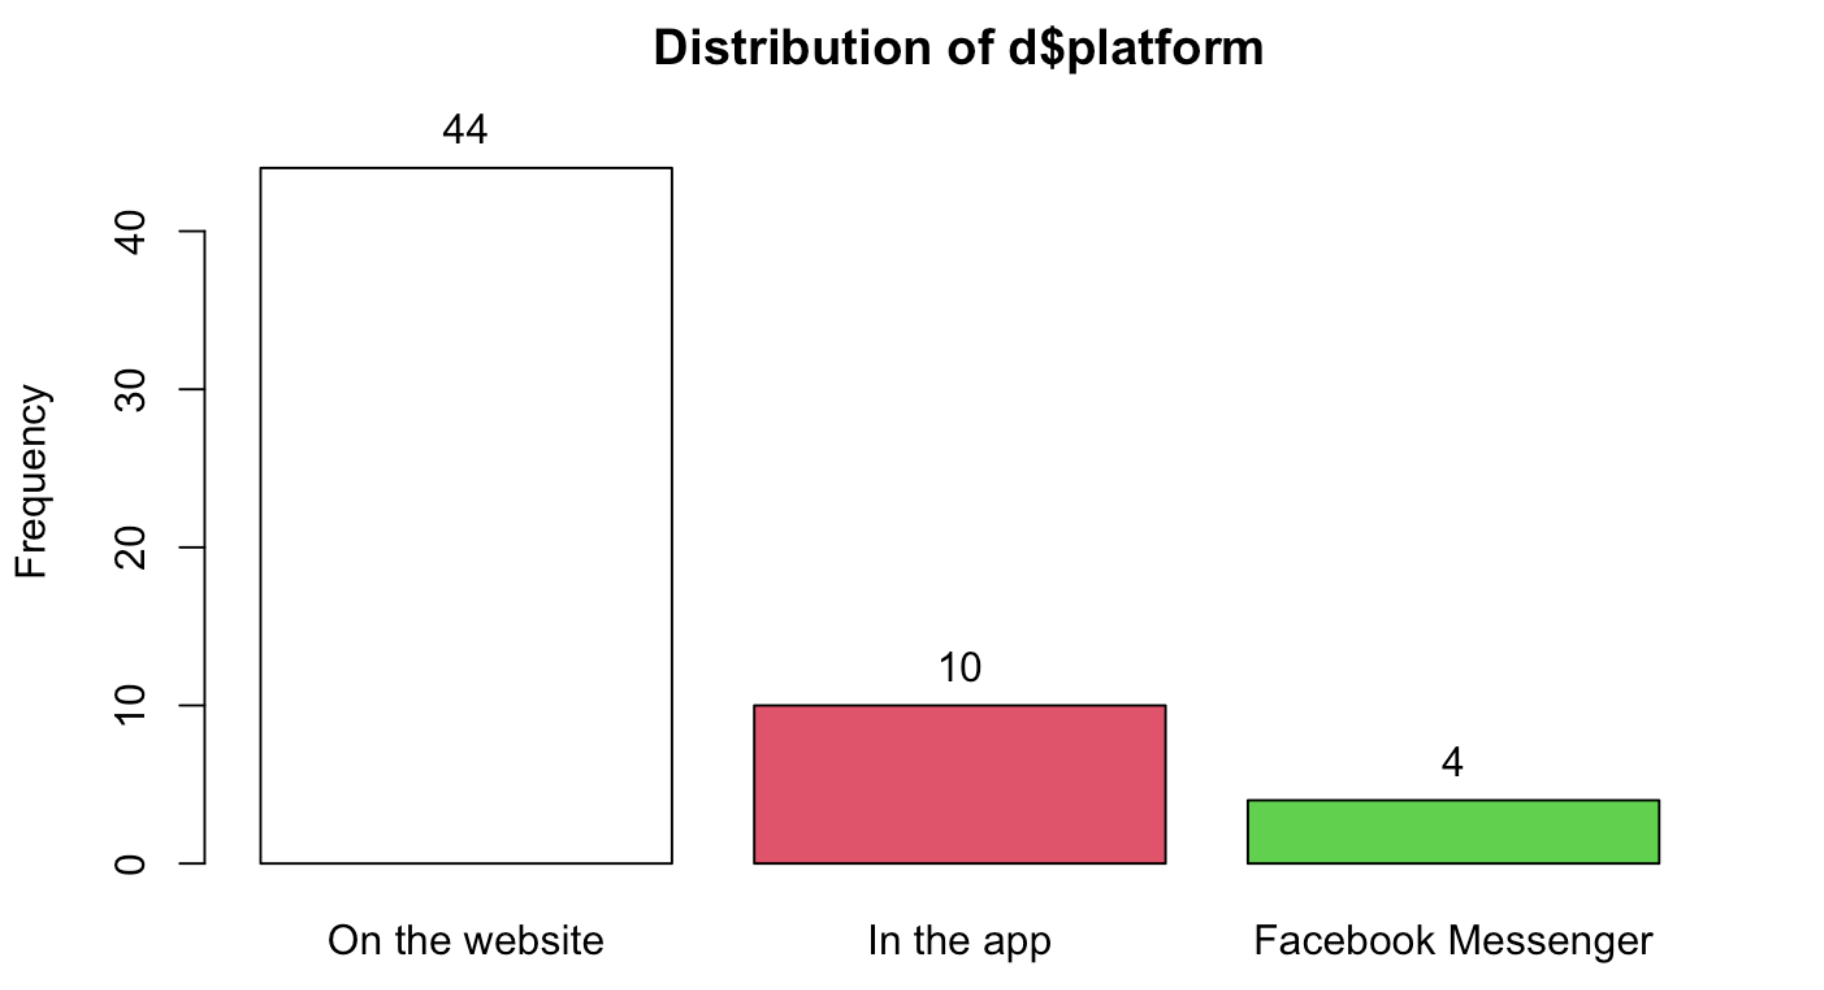
\includegraphics[width=\linewidth]{../LaTeX/Figures/Environments/PlatformPlot.png}
	\caption{The distribution of the platform variable.}\label{fig:platformPlot}
	\endminipage\hfill
	\minipage{0.30\textwidth}
	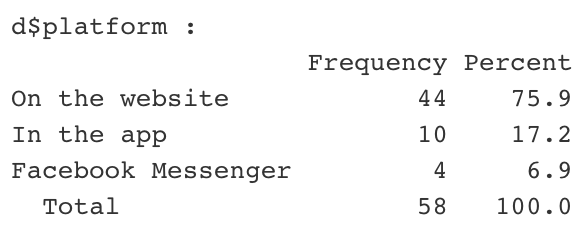
\includegraphics[width=\linewidth]{../LaTeX/Figures/Environments/PlatformFreq.png}
	\caption{A frequency table of all the entries' used platforms to interact with the chatbot.}\label{fig:platformFreq}
	\endminipage\hfill
\end{figure}

\FloatBarrier
\subsection{Comparative Study}
\subsubsection{Business view (interviews)}
\begin{table}[htbp!]
	\centering
	\resizebox{\textwidth}{!}{%
		\begin{tabular}{|lllll|}
			\hline
			\multicolumn{5}{|c|}{\textbf{The current state of the customer service chatbot}} \\ \hline
			\multicolumn{1}{|l|}{} &
			\multicolumn{1}{l|}{Proximus} &
			\multicolumn{1}{l|}{Telenet} &
			\multicolumn{1}{l|}{T-Mobile} &
			KPN \\ \hline
			\multicolumn{1}{|l|}{\begin{tabular}[c]{@{}l@{}}Supported task \\ categories\end{tabular}} &
			\multicolumn{1}{l|}{FAQ} &
			\multicolumn{1}{l|}{FAQ} &
			\multicolumn{1}{l|}{\begin{tabular}[c]{@{}l@{}}FAQ, Sales (add-ons\\ like Deezer and \\ other video services)\end{tabular}} &
			FAQ \\ \hline
			\multicolumn{1}{|l|}{\begin{tabular}[c]{@{}l@{}}Supported \\ platforms\end{tabular}} &
			\multicolumn{1}{l|}{\begin{tabular}[c]{@{}l@{}}Website,\\ Messenger,\\ Proximus-app\end{tabular}} &
			\multicolumn{1}{l|}{Messenger} &
			\multicolumn{1}{l|}{Website and app} &
			Website and app\\ \hline
			\multicolumn{1}{|l|}{\begin{tabular}[c]{@{}l@{}}Supported \\ languages\end{tabular}} &
			\multicolumn{1}{l|}{\begin{tabular}[c]{@{}l@{}}Dutch, French,\\  English\end{tabular}} &
			\multicolumn{1}{l|}{\begin{tabular}[c]{@{}l@{}}Dutch, French,\\  English\end{tabular}} &
			\multicolumn{1}{l|}{Dutch} &
			Dutch \& English \\ \hline
			\multicolumn{1}{|l|}{\begin{tabular}[c]{@{}l@{}}Most common \\ user group\end{tabular}} &
			\multicolumn{1}{l|}{No information} &
			\multicolumn{1}{l|}{\begin{tabular}[c]{@{}l@{}}Younger people \\ and adults\\ (\textless{}= 40 years)\end{tabular}} &
			\multicolumn{1}{l|}{\begin{tabular}[c]{@{}l@{}}T-Mobile = adults\\ Tele2 = younger\\ people\end{tabular}} &
			Adults \\ \hline
			\multicolumn{1}{|l|}{\begin{tabular}[c]{@{}l@{}}Supported\\ questions\end{tabular}} &
			\multicolumn{1}{l|}{\begin{tabular}[c]{@{}l@{}}Yes/no, direct \\ \& vague \\ questions\end{tabular}} &
			\multicolumn{1}{l|}{\begin{tabular}[c]{@{}l@{}}Only predefined\\ scenarios\end{tabular}} &
			\multicolumn{1}{l|}{\begin{tabular}[c]{@{}l@{}}Yes/no, direct \& \\ vague questions\end{tabular}} &
			\begin{tabular}[c]{@{}l@{}}Yes/no, direct \& \\ vague questions\end{tabular} \\ \hline
		\end{tabular}%
	}
	\caption{Overview of the current state of the customer service chatbots}
	\label{tab:currentState}
\end{table}
\ul{Supported task categories}\\
Later on, Proximus wants to develop their chatbot further into a proactive salesman with the aim of offering the best action or promotion. Complaints are forwarded by the bot directly to a live agent.\\
\break
Telenet used to have two chatbots, AskHugo and AskPlay. AskHugo was a bot that tried to convince customers to buy a Hugo subscription, AskPlay gave recommendations on which movies/series to watch. However, both chatbots were shut down because the \acrshort{roi} was too low. Now they have an FAQ bot that only supports predefined scenarios and is mainly used to gather information for the agents.\\
\break
T-Mobile's\footnote{T-Mobile has merged with Tele2 since January 2019. The Tele2 brand has continued to exist and is now a part of T-Mobile. The management of Tele2's chatbot is also done by T-Mobile, these chatbots both use the same underlying system so both chatbots have the same operations.} chatbot can also guide the customer in choosing the right subscription or device. This way, T-Mobile tries to keep as much "trivial" work away from the physical agents, because the explicit purchase of a specific subscription/device is only done through them. Complaints are partly handled by the bot, it will ask if the customer has already spoken to an employee about this, if this has happened, then the chatbot will give the procedure to file a complaint.\\
\break
At the chatbot of KPN, in case of complaints, the customer is redirected to a live chat; the bot's only function here is to gather customer information. Selling products and services is not offered in the bot because that is not yet technically possible, the bot only serves as a proactive assistant, if the customer has been in the shop for a while, the bot will ask if the customer needs help.\\
\break
\ul{Supported platforms}\\
Telenet only offers its chatbot through Facebook Messenger, but this is integrated into their website and app. Communication through WhatsApp is also possible, but this is only an auto-reply system. In the bot of T-Mobile, there is a difference between the platforms, on the website all services are offered, but in the application the chatbot is mainly focused on questions about mobile services. The bot recognises if the customer asks a question about another service, he will then be redirected. KPN basically only offers their chatbot on their website, but in the app it is also available through a webview. If the customer then consults the chatbot in the app, this is actually the chatbot on the website.\\
\break
\ul{Supported languages}\\
If the Proximus bot is addressed in a different language, the underlying \acrshort{ai} system will recognise that this language is not supported, and the bot will then choose to continue the conversation in English. When the bot of T-Mobile is used in another language, the customer is redirected to an agent. The English variant of KPN's bot has far fewer functions; it will redirect the customer to the right page on the website or continue the conversation with an agent. According to KPN, there is no need in the Netherlands to offer the chatbot in other languages (see Appendix A.4.1). \\
\break
\ul{Most common user group}\\
Proximus' broad customer base explains the big spread of its users, as they offer services that are used by young people, adults and the elderly. Telenet's most common user group can be explained because their bot can only be accessed via social media. T-Mobile only has insight into the bot users that have been identified (users who are logged in to their account). T-Mobile also anticipates on the age group by adjusting the chat style; in the Tele2 bot, more hashtags and emojis are used, in the T-Mobile bot this is more formal. KPN uses a neutral chat style in their bot, they don't want to address a specific age group.\\
\break
\ul{Supported type of questions}\\
For every bot except Telenet, the yes/no questions are supported. The treatment of the direct and vague is also in the same line in the different bots. Whenever a question is too vague, the bot will continue to ask until the various missing values have been filled in. In the T-Mobile bot, it was mentioned that there is a limit to the number of times that a certain missing value can be queried. If the bot needs to re-ask a certain number of times before it can provide an answer, the chat will be redirected to a live agent to avoid user frustration. To address the same issue, KPN is using a button where the user can indicate whether they mean something different or have a different question. Telenet's chatbot can't interpret anything, you have to work with the buttons provided by the chatbot.\\
\begin{table}[htbp!]
	\centering
	\resizebox{\textwidth}{!}{%
		\begin{tabular}{|lllll|}
			\hline
			\multicolumn{5}{|c|}{\textbf{The benefits that the company derives from the presence of the chatbot}} \\ \hline
			\multicolumn{1}{|l|}{} &
			\multicolumn{1}{l|}{Proximus} &
			\multicolumn{1}{l|}{Telenet} &
			\multicolumn{1}{l|}{T-Mobile} &
			KPN \\ \hline
			\multicolumn{1}{|l|}{\begin{tabular}[c]{@{}l@{}}Supported\\ services\end{tabular}} &
			\multicolumn{1}{l|}{\begin{tabular}[c]{@{}l@{}}- Retrieve pincode\\ - Outstanding\\ invoice amount\\ - Retrieve status\\ of your subscription\\ and services\end{tabular}} &
			\multicolumn{1}{l|}{- Only support} &
			\multicolumn{1}{l|}{\begin{tabular}[c]{@{}l@{}}- Retrieve customer\\ information (client\\ number, \acrshort{puk} code\\ , etc.)\\ -Adjust personal\\ settings (e.g.\\ deactivate extra\\ costs if a service \\ number calls)\\ - Buy add-ons (e.g.\\ mobile data bundle)\\  - Manages \\ workforce of agents\end{tabular}} &
			\begin{tabular}[c]{@{}l@{}}- Preparer for\\ agents (making\\ their conversation\\ shorter)\\ - Guide to lead\\ customer to right\\ place on website\end{tabular} \\ \hline
			\multicolumn{1}{|l|}{\begin{tabular}[c]{@{}l@{}}Reduction of\\ employee\\ workload\end{tabular}} &
			\multicolumn{1}{l|}{\begin{tabular}[c]{@{}l@{}}No data because of\\ confidential \\ information\end{tabular}} &
			\multicolumn{1}{l|}{\begin{tabular}[c]{@{}l@{}}No data because\\ of confidential\\ information\end{tabular}} &
			\multicolumn{1}{l|}{\begin{tabular}[c]{@{}l@{}}25\% of the question\\ can not be answered\\ in the chatbot\end{tabular}} &
			\begin{tabular}[c]{@{}l@{}}The chatbot takes\\ over 25\% of the\\ work\end{tabular} \\ \hline
			\multicolumn{1}{|l|}{\begin{tabular}[c]{@{}l@{}}Customer's\\ willingness to\\ use chatbot\end{tabular}} &
			\multicolumn{1}{l|}{\begin{tabular}[c]{@{}l@{}}No data because of \\ confidential \\ information\end{tabular}} &
			\multicolumn{1}{l|}{\begin{tabular}[c]{@{}l@{}}65\% of the users\\ are willing to go\\ through the\\ whole flow\end{tabular}} &
			\multicolumn{1}{l|}{No data available} &
			\begin{tabular}[c]{@{}l@{}}20\% of the users\\ do not want to\\ use the chatbot \end{tabular} \\ \hline
			\multicolumn{1}{|l|}{\begin{tabular}[c]{@{}l@{}}Negative\\ influences\end{tabular}} &
			\multicolumn{1}{l|}{\begin{tabular}[c]{@{}l@{}}- Frustration\\ because of bad \\ experience and\\ prejudice\end{tabular}} &
			\multicolumn{1}{l|}{\begin{tabular}[c]{@{}l@{}}- Frustration\\ because of the\\ change to a new\\ platform\end{tabular}} &
			\multicolumn{1}{l|}{\begin{tabular}[c]{@{}l@{}}- Frustration because\\ of bad experience\\ and prejudice\end{tabular}} &
			\begin{tabular}[c]{@{}l@{}}No data available\\ because of \\ confidential\\ information\end{tabular} \\ \hline
		\end{tabular}%
	}
	\caption{Overview of the benefits that companies derive from the presence of the chatbot}
	\label{tab:benefits}
\end{table}
\break
\ul{Supported services}\\
The purpose of Proximus' chatbot is to offer solutions, not instructions such as "for that task, you can go to this web page". At T-Mobile, the sales contracts are not handled in the chatbot because the sales department does not want it to deal with their sales strategies.\\
\break
\ul{Reduction of employee workload}\\
Proximus said that not everything in customer service was covered, so for some issues customers are redirected to an employee. The chatbot of Telenet reduces the workload, but the impact is still limited. T-Mobile's numbers can be explained by poor language use by the customer or the complexity and specificity of the question. The results of KPN's chatbot can be explained as the bot does not have enough knowledge to answer the question; for some services, such as cancelling subscriptions or complaints, the customer is always referred to a member of staff. It is estimated that about a quarter (25\%) of the agents' work is taken over by the chatbot.\\
\break
\ul{Customer's willingness to use chatbot}\\
The willingness to use the chatbot is examined by each company on the basis of feedback, with feedback one must also take into account voluntary response bias, customers who are not satisfied with certain services will give feedback more quickly than others.\\
\break
At Proximus the satisfaction lies in both camps, there are customers who are very satisfied with the chatbot, but there are also customers who think it is very bad.\\ 
\break
In the bot of Telenet, the reason why the remaining 35\% drop out is explained by a bad previous experience with a similar chatbot.\\ 
\break
T-Mobile asks their customers for feedback after a conversation with a chatbot. Analyses showed that the majority of responses ultimately had to call an agent to solve their problem. What T-Mobile also does to gain more insight into their customers is to work with personas. These are linked to possible customer profiles where they map out the corresponding requirements of the customer.\\ 
\break
At KPN, the number of direct calls (telephone) to a physical agent would be up higher, to an order of about ten, than with the chatbot. This means that there are ten times more calls than chats.\\
\break
\ul{Negative influences}\\
Proximus sees mainly negative influences in the form of customers who are frustrated. The frustration arises when the chatbot does not understand the customer properly and goes the wrong way, this demotivates the customer to reuse the bot. Customers who are already frustrated by services that do not work properly should be taken into account, if these customers then come into contact with a chatbot it will not help their mood.\\
\break
Telenet experiences similar scenarios, it was further explained that it can be frustrating for customers to switch to a new platform, namely from 100\% helpdesk to a chatbot. According to Ms Portolani, some customers expect that a chatbot can interpret in the same way as an agent.\\
\break
T-Mobile has the same negative aspects as Proximus, they try to solve this by applying a limited form of sentiment analysis. If they measure that a customer is communicating in a frustrated way, they will forward this customer to an agent.\\
\break
At KPN, different metrics are used. For instance, the \gls{nps} measures the extent to which customers would recommend the company to acquaintances. The \acrfull{ces} measures how much effort it took to find the answer to the question. The final metric measured is the \acrfull{gcr}, which tells more about how well the customer was helped. The results of these metrics were not shared due to confidential information.\\
\break
\begin{longtable}[c]{|lllll|}
	\hline
	\multicolumn{5}{|c|}{\textbf{The business value (revenue, reduced costs) realised by the chatbot}} \\ \hline
	\endhead
	%
	\multicolumn{1}{|l|}{} &
	\multicolumn{1}{l|}{Proximus} &
	\multicolumn{1}{l|}{Telenet} &
	\multicolumn{1}{l|}{T-Mobile} &
	KPN \\ \hline
	\multicolumn{1}{|l|}{\begin{tabular}[c]{@{}l@{}}Increased \\ revenue\end{tabular}} &
	\multicolumn{1}{l|}{\begin{tabular}[c]{@{}l@{}}- No direct \\ revenue because \\ ROI is not\\ yet determined\\ - Chatbot directly\\ ensures they have\\ to spend less on\\ human helpdesk\\ agents\end{tabular}} &
	\multicolumn{1}{l|}{\begin{tabular}[c]{@{}l@{}}- No picture of\\ how much extra\\ revenue\\ - They have\\ fewer costs to\\ spent on\\ physical agents\end{tabular}} &
	\multicolumn{1}{l|}{\begin{tabular}[c]{@{}l@{}}- No concrete\\ figures, because\\ it is not measured\\ - Extra business\\ value is created\\ because fewer \\ costs to spent \\ on physical agents\end{tabular}} &
	\begin{tabular}[c]{@{}l@{}}- No concrete\\ figures, because \\ it is not measured\\ - Extra business\\  value is created\\ because fewer \\ costs to spent on \\ physical agents\end{tabular} \\ \hline
	\multicolumn{1}{|l|}{Availability} &
	\multicolumn{1}{l|}{\begin{tabular}[c]{@{}l@{}}- 24/7 available\\ - Follow-up on \\ social media is \\ always possible\\ - Follow-up on the\\ website and in the\\ app is only \\ possible if user is \\ authenticated\end{tabular}} &
	\multicolumn{1}{l|}{\begin{tabular}[c]{@{}l@{}}- 24/7 available\\ - Follow-up is\\ always possible\\ because they\\ only use social\\ media\end{tabular}} &
	\multicolumn{1}{l|}{\begin{tabular}[c]{@{}l@{}}- 24/7 available\\ - Conversation is \\ not tracked, so the \\ customer will have \\ to consult the \\ chatbot again \\ during opening \\ hours if the \\ question cannot\\  be answered by \\ the chatbot\end{tabular}} &
	\begin{tabular}[c]{@{}l@{}}- 24/7 available\\ - Conversation is \\ not tracked, so \\ the customer will \\ have to consult \\ the chatbot again \\ during opening \\ hours if the \\ question cannot \\ be answered by \\ the chatbot\end{tabular} \\ \hline
	\multicolumn{1}{|l|}{\begin{tabular}[c]{@{}l@{}}Costs \& \\ biggest \\ cost items\end{tabular}} &
	\multicolumn{1}{l|}{\begin{tabular}[c]{@{}l@{}}- Costs depend\\ mainly on the\\ platform and the\\ size (number of\\ questions / \\ scenarios the bot \\ can handle)\\  of the chatbot\\ Biggest cost \\ items:\\ - Per incoming\\ chat, the NLP is\\ triggered, this \\ costs around \\ 1cent/chat\\ - The team behind\\ the chatbot, this \\ consists of in-\\ house frontend \\ and backend \\ developers,\\ configuration / \\ conversation \\ designers(via \\ consultancy and \\ cost about €400/\\ day) and an \\ engineer that \\ trains and corrects \\ the NLP\end{tabular}} &
	\multicolumn{1}{l|}{\begin{tabular}[c]{@{}l@{}}- They use a\\ pay-as-you-go\\ service, specific\\ costs could not\\ be shared\\ because of\\ confidential\\ information\\ Biggest cost\\ items:\\ - Hosting of the\\ chatbot\\ - Team behind\\ the development,\\ it consists of a\\ data scientist,\\ developer,\\ functional analyst\\ and a product\\ owner. It was\\ reported that \\ most of the costs \\ goes\\ to the team.\end{tabular}} &
	\multicolumn{1}{l|}{\begin{tabular}[c]{@{}l@{}}Specific costs could\\ not be shared because\\ of confidential \\ information\\ Biggest cost items:\\ - They have a\\ significant amount of\\ running costs because\\ the run their chatbot\\ in the cloud\\ - They use \\ Dialogflow (Google),\\  this tool contains \\ a CMS and\\ you can apply AI in\\ it\\ - Running costs\\ consist of \\ classification API, \\ database operations\\ and running the \\ engines to keep \\ everything working\\ - Largest part of the \\ costs go to the team \\ behind the bot, it \\ consists of two \\ developers, \\ full-stack developers \\ from India (quantity \\ unknown),\\ two AI trainers and\\ two conversation\\ designers\end{tabular}} &
	\begin{tabular}[c]{@{}l@{}}- They buy the \\ chatbot services \\ from another \\ company\\ -No specific data \\ on the costs could \\ be shared because \\ of confidential\\ information\\ Biggest cost items:\\ - The price they \\ pay\\ to the company\\ that created \\ and hosts the \\ chatbot\\ - Two teams that \\ work on the bot (\\ conversational\\ designers, product\\ owners, ...)\end{tabular} \\ \hline
	\caption{Overview of the business value (revenue, reduced costs) that are realised by the chatbots}
	\label{tab:businessValue}\\
\end{longtable}
Every chatbot that was questioned is available 24/7, but there is a difference in the handling of questions that cannot be solved by the chatbot during non-opening hours.\\
\break
\begin{longtable}[c]{|lllll|}
	\hline
	\multicolumn{5}{|c|}{\textbf{The future vision of the chatbot}} \\ \hline
	\endhead
	%
	\multicolumn{1}{|l|}{} &
	\multicolumn{1}{l|}{Proximus} &
	\multicolumn{1}{l|}{Telenet} &
	\multicolumn{1}{l|}{T-Mobile} &
	KPN \\ \hline
	\multicolumn{1}{|l|}{\begin{tabular}[c]{@{}l@{}}Focal points\\ for the \\ future\end{tabular}} &
	\multicolumn{1}{l|}{\begin{tabular}[c]{@{}l@{}}- Future view was\\ mostly confidential\\ - In general, they\\ are looking to \\ automate their \\ services and be \\ stronger in terms \\ of conversation\\ - Are looking\\ further into voice\\ control (next\\ channel they will\\ capitalise on)\\ - Reducing the\\ buttons in their \\ bot, goal is to be \\ as conversational \\ as possible\\ - Are looking into\\ computer vision\\ - In the long term,\\ they want to\\ integrate the bot\\ with Alexa, \\ Google Home, \\ etc.\end{tabular}} &
	\multicolumn{1}{l|}{\begin{tabular}[c]{@{}l@{}}- Are currently\\ working on a \\ platform in \\ which the \\ chatbot can\\ take more tasks\\ and answer \\ questions\\ independently\\ - They want to\\ add sentiment\\ analysis\\ - Branding the\\ new chatbot to\\ make it known\\ to their future\\ users\\ - They want to\\ add text\\ prediction to the\\ tool of the \\ human agents\end{tabular}} &
	\multicolumn{1}{l|}{\begin{tabular}[c]{@{}l@{}}- They want to offer\\ the chatbot more\\ proactively on the\\ website\\ - Making the chatbot\\ available in more \\ languages with a \\ translate API (both\\ parties can then use\\ the bot in their own\\ language)\\ - Add asynchronous\\ messaging\end{tabular}} &
	\begin{tabular}[c]{@{}l@{}}- Making the bot\\ available in more\\ places (presence\\ on social media\\ as Facebook \\ Messenger and \\ WhatsApp)\\ - Harmonise the\\ entire \\ communication \\ with the customer\\ (if the customer \\ send them via \\ WhatsApp,\\ they want to be \\ aware of this \\ conversation\\ if the customer\\ contacts them via \\ another platform\end{tabular} \\ \hline
	\multicolumn{1}{|l|}{\begin{tabular}[c]{@{}l@{}}Additional\\ chatbot-\\ features\end{tabular}} &
	\multicolumn{1}{l|}{\begin{tabular}[c]{@{}l@{}}Uses AI to classify\\ the question or \\ statement, \\ once this \\ is classified a \\ rule-based \\ approach is used\end{tabular}} &
	\multicolumn{1}{l|}{\begin{tabular}[c]{@{}l@{}}Only uses a \\ rule-based \\ approach\end{tabular}} &
	\multicolumn{1}{l|}{\begin{tabular}[c]{@{}l@{}}Uses AI to classify\\ the question or \\ statement, once this\\ is classified a \\ rule-based approach\\ is used\end{tabular}} &
	\begin{tabular}[c]{@{}l@{}}Uses AI to classify\\ the question or \\ statement, once this\\ is classified a \\ rule-based \\ approach is used\end{tabular} \\ \hline
	\multicolumn{1}{|l|}{\begin{tabular}[c]{@{}l@{}}Source of\\ knowledge\\ to improve\\ chatbot\end{tabular}} &
	\multicolumn{1}{l|}{\begin{tabular}[c]{@{}l@{}}They use \\ benchmarking,\\ marketing studies,\\ check-ins with \\ other companies, \\ research in papers\\ and participation\\ in many \\ conferences \\ to gather extra \\ information on\\ relevant topics\end{tabular}} &
	\multicolumn{1}{l|}{\begin{tabular}[c]{@{}l@{}}- Are using data\\ analysis\\ - They look at\\ the experience \\ of their agents\end{tabular}} &
	\multicolumn{1}{l|}{\begin{tabular}[c]{@{}l@{}}- Uses data analysis,\\ each conversation is\\ logged and they can\\ query to gather \\ information on \\ specific topics\\ - Customer feedback\\ is taken into account,\\ in the conversations\\ that went well, they\\ take the common\\ features and use \\ them to standardize \\ this in the \\ conversation design,\\ for the bad\\ conversations, they\\ look for aspects that\\ they can further \\ improve\end{tabular}} &
	\begin{tabular}[c]{@{}l@{}}- Main focus on \\ data analysis to \\ continuously \\ review how they \\ can improve the \\ conversations\end{tabular} \\ \hline
	\caption{Overview of the future vision of the different chatbots}
	\label{tab:futureVision}\\
\end{longtable}
Proximus is looking into integrating computer vision, for example, if a picture of an invoice is sent in the bot, it can automatically recognise the different elements.\\
\break
Telenet is focusing on automating certain things the agents work with, they want to add text prediction so when the agent starts typing they will automatically prefill things so the agent does not have to type everything themselves.\\
\break
T-Mobile is working on adding asynchronous messaging, which means that if it is necessary to chat with an agent, no synchronous connection is needed, and the flow of the chat will continue exactly as it started with the chatbot. The latter will also ensure that customers do not need to send their question again if they have consulted the chatbot outside of helpdesk opening hours.

\subsubsection{Customer view (survey)}
In this part, a comparison will be drawn between the different companies in accordance to the business interview and gathered data in the survey. Because Orange, T-Mobile and KPN did not get enough responses to be viewed on their own, these three providers will be grouped together in the group 'others'.\\
\break
Next up, the task categories. Because the interview showed that chatbots are not yet equipped to deal with both complaints as well as sales questions, these two will not be included in the comparative study. For personal questions, there are not enough entries to view this as it is own category. The focus will therefor be on FAQ questions.\\
\break
All graphs will be presented as follows: Telenet on the left, Proximus in the middle and the 'others' on the right.\\
\break
\ul{Attribute 1: Execute the requested task}\\
\break
Looking at how the chatbots performed when solving a task, both Telenet and Proximus seem to have a split customer base where around 50\% is happy and 50\% is not. When looking at the others, there is a clear happiness about how the chatbot performed (Figure \ref{fig:Q1}).\\
\begin{figure}[!htb]
	\centering
	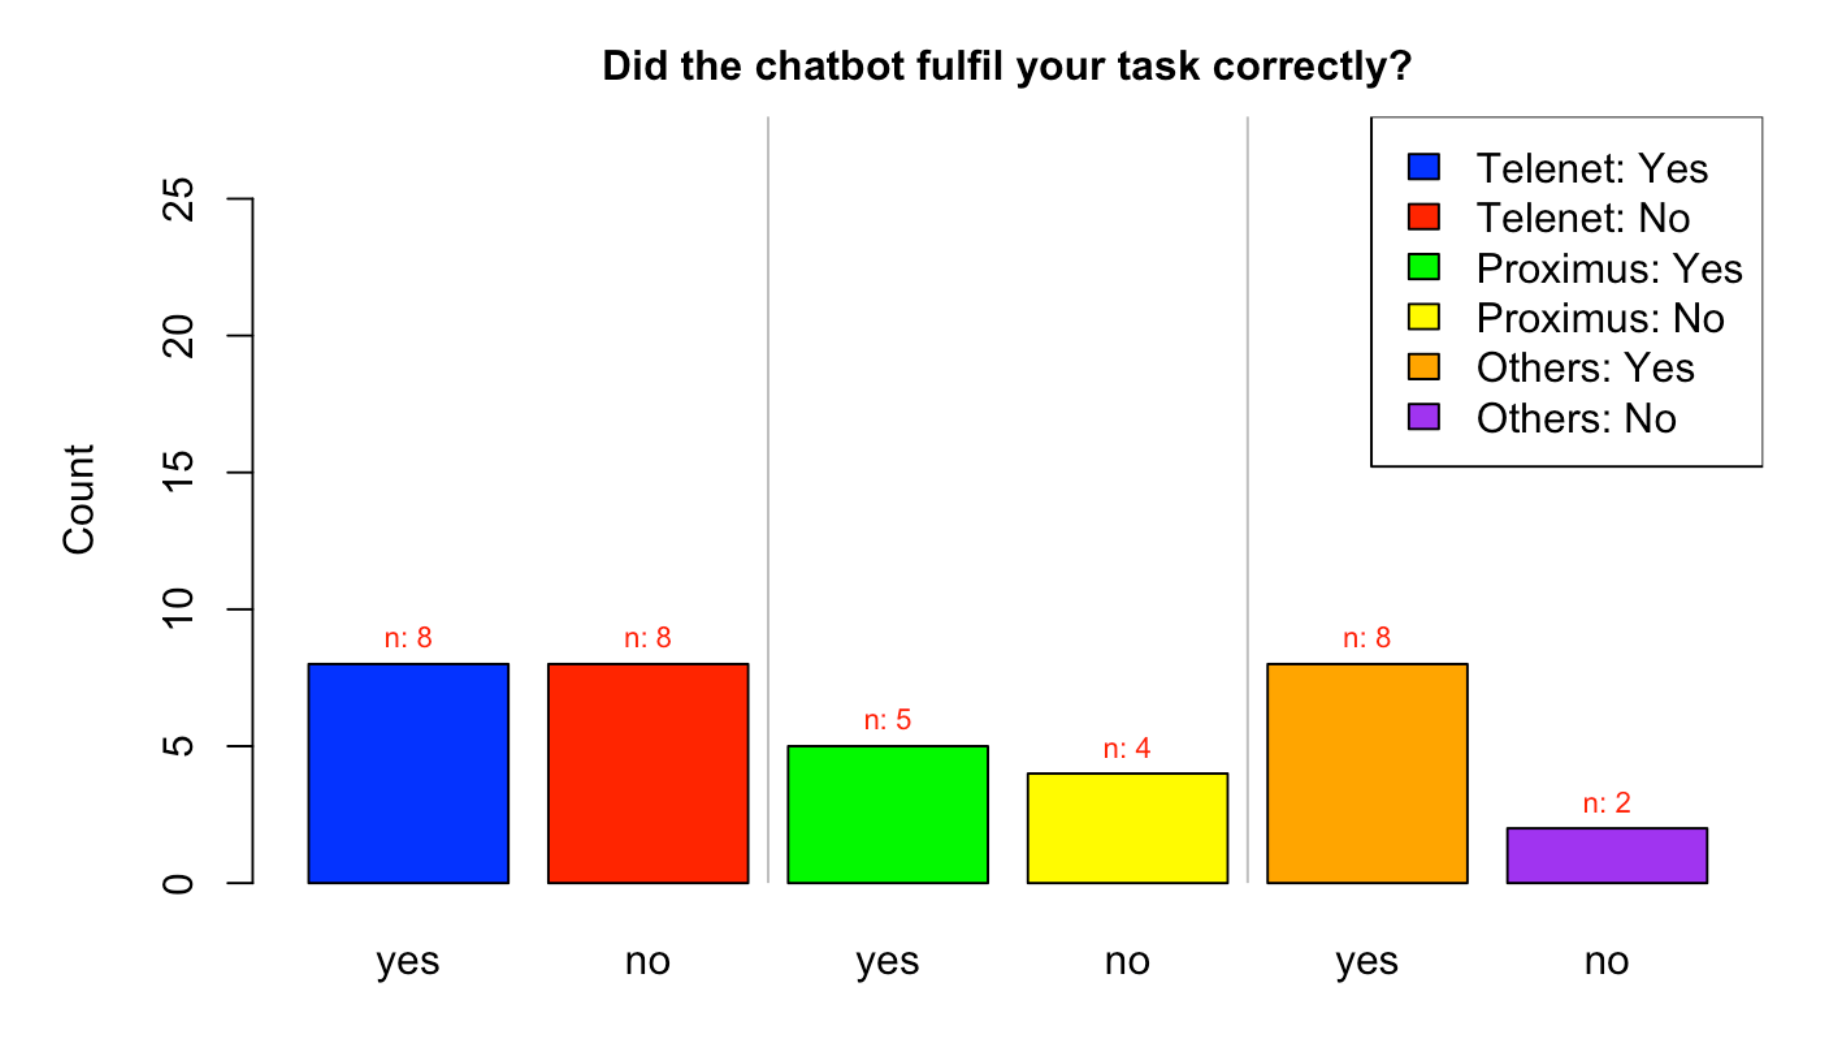
\includegraphics[width=375pt]{../LaTeX/Figures/Comparative/Q1.png}
	\caption{Responses about the functional question for \acrshort{qa} 1, question 1.}\label{fig:Q1}
\end{figure}
\break
Looking at the counter part of the previous question, there is even more discontent with Proximus. The results for Telenet and the others confirm the previous findings (Figure \ref{fig:DQ1}).
\begin{figure}[!htb]
	\centering
	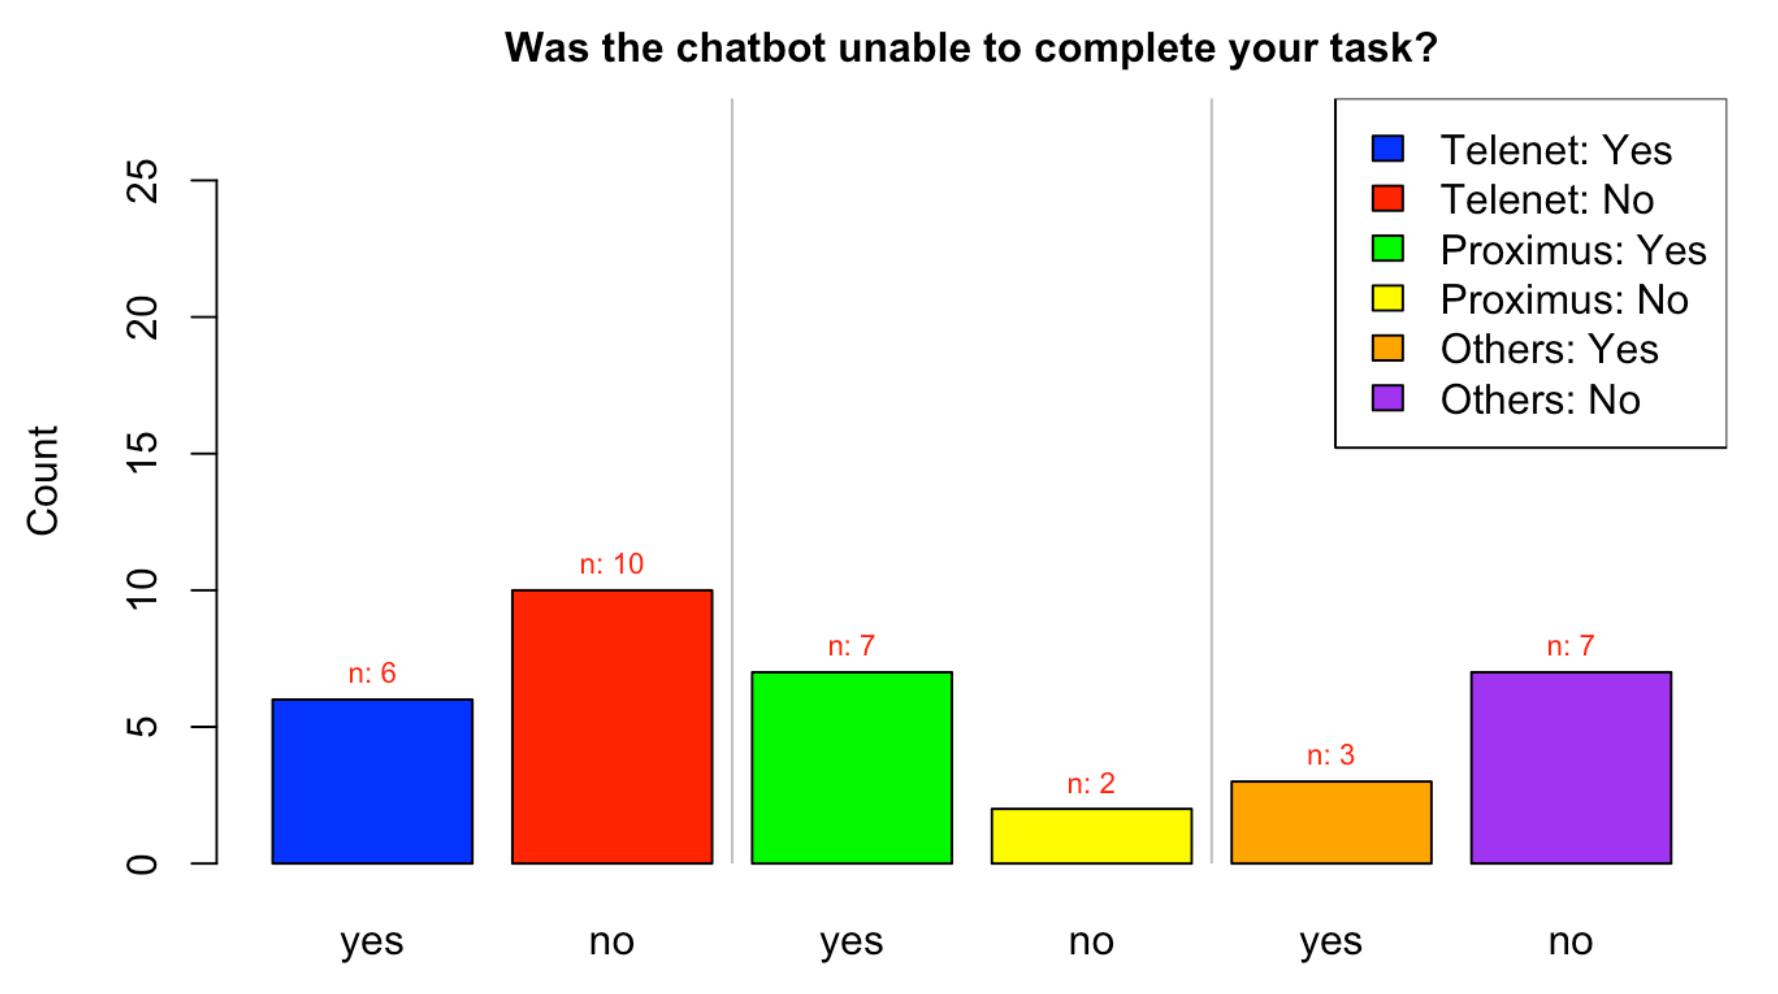
\includegraphics[width=375pt]{../LaTeX/Figures/Comparative/DQ1.png}
	\caption{Responses about the dysfunctional question for \acrshort{qa} 1, question 1.}\label{fig:DQ1}
\end{figure}
\break
Looking at the results whether the chatbot needed help from an agent to complete it's task, there again is almost a 50-50 split for Telenet and Proximus whereas the others did better again (Figure \ref{fig:Q1b}).\\
\begin{figure}[!htb]
	\centering
	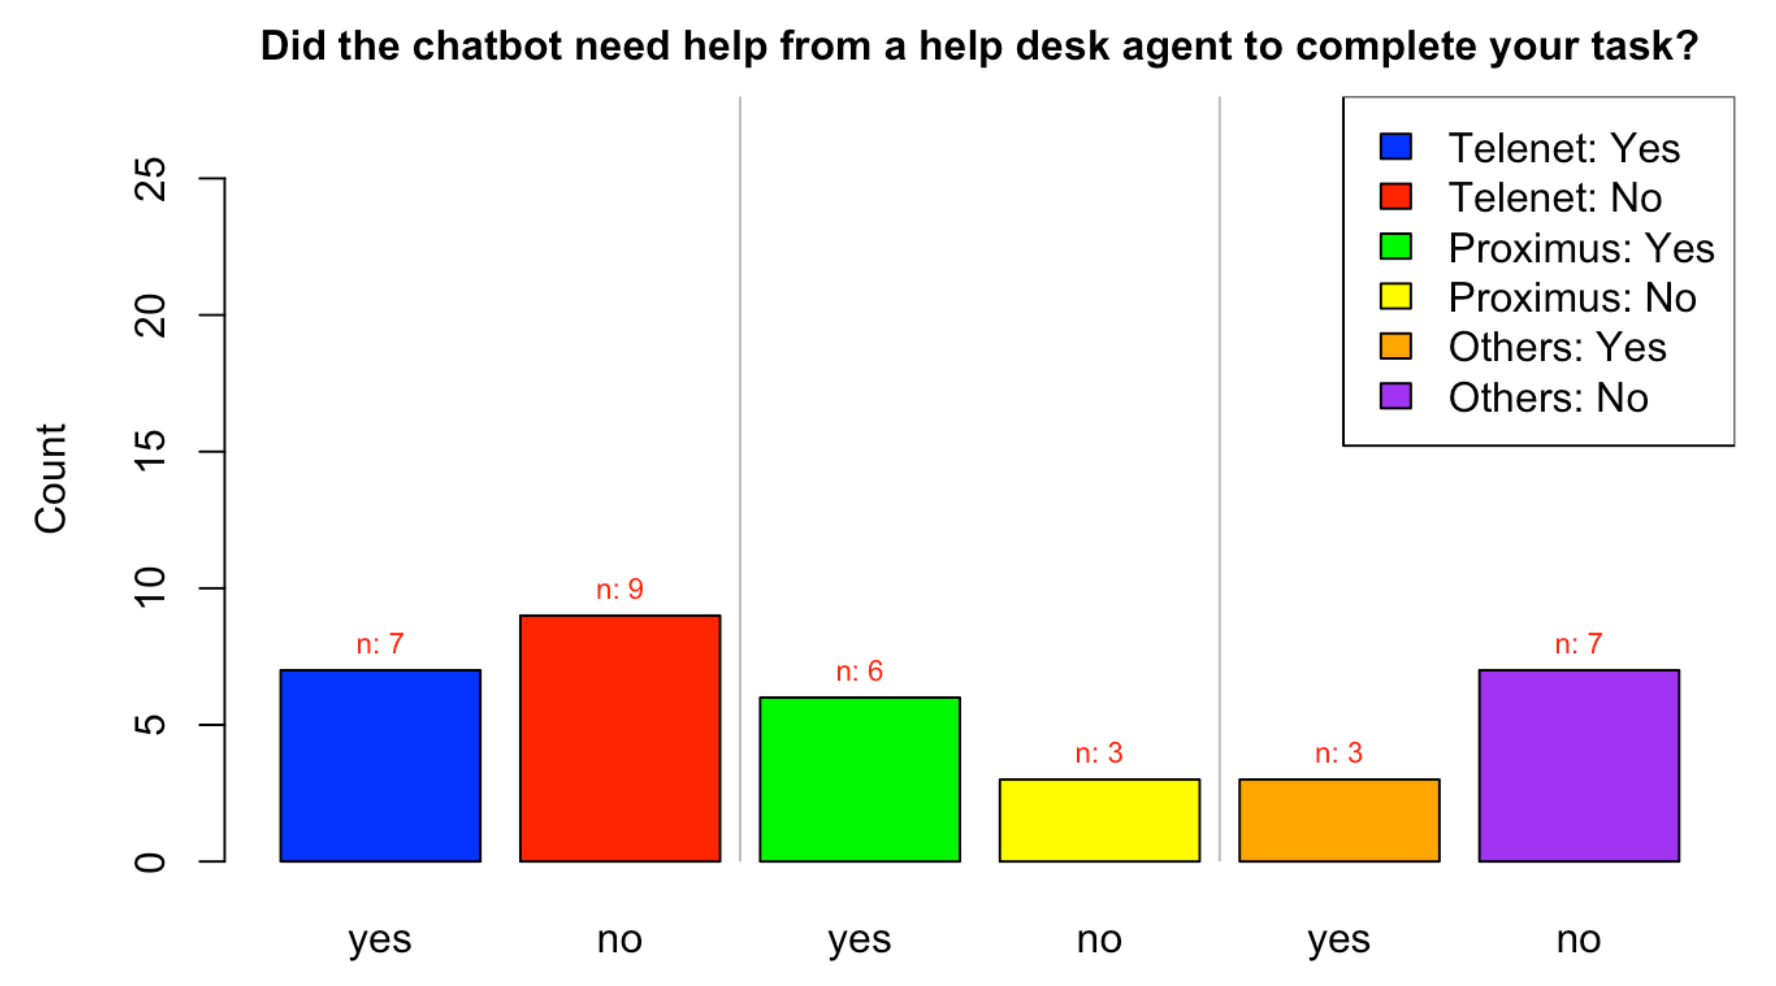
\includegraphics[width=375pt]{../LaTeX/Figures/Comparative/Q1b.png}
	\caption{Responses about the functional question for \acrshort{qa} 1, question 2.}\label{fig:Q1b}
\end{figure}
\break
The dysfunctional version of the previous question confirms these findings (Figure \ref{fig:DQ1b}).\\
\begin{figure}[!htb]
	\centering
	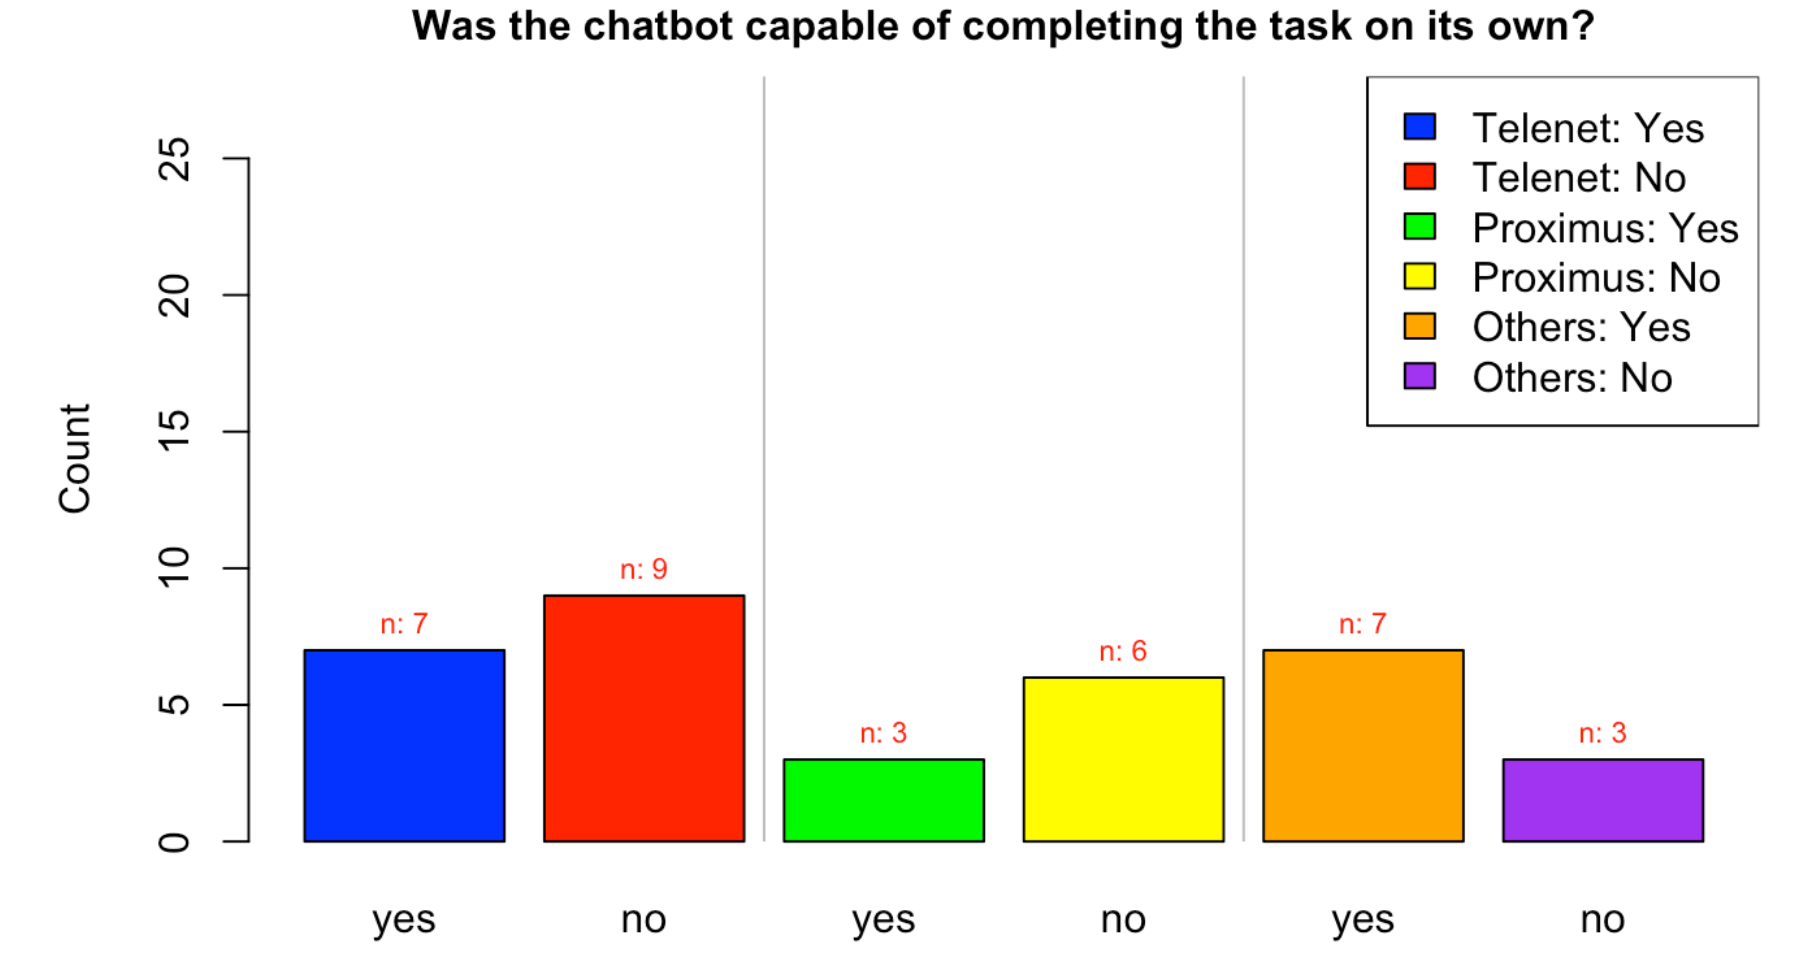
\includegraphics[width=375pt]{../LaTeX/Figures/Comparative/DQ1b.png}
	\caption{Responses about the dysfunctional question for \acrshort{qa} 1, question 2.}\label{fig:DQ1b}
\end{figure}
\break
A third question to gauge the capabilities of the chatbot to execute the requested task was about the expectations of the chatbot and if it lived up to them. The results show that the chatbot mostly lived up to expectations, even though it could not solve the task it was given (Figure \ref{fig:Q1c}).\\
\begin{figure}[!htb]
	\centering
	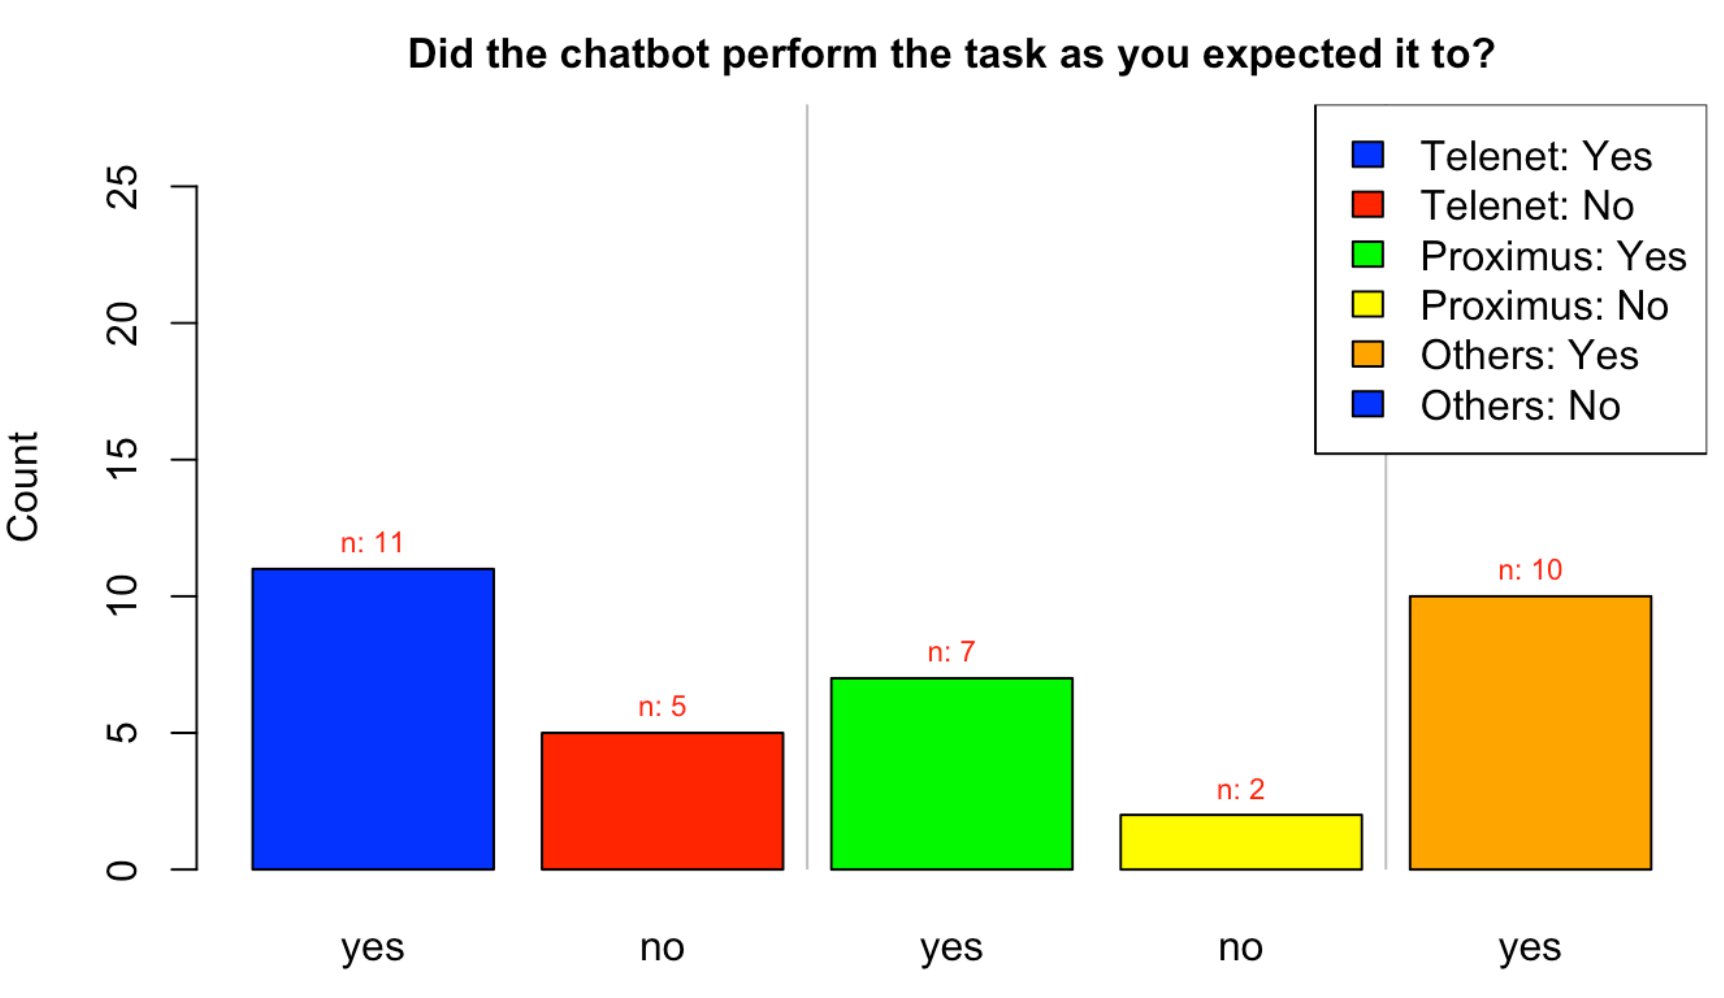
\includegraphics[width=375pt]{../LaTeX/Figures/Comparative/Q1c.png}
	\caption{Responses about the functional question for \acrshort{qa} 1, question 3.}\label{fig:Q1c}
\end{figure}
\break
A fourth and final question asked if the user could solve the problem after interacting with the chatbot. For Proximus, there was some pushback but for Telenet and the others, the majority voted yes (Figure \ref{fig:DQ1c}).\\
\begin{figure}[!htb]
	\centering
	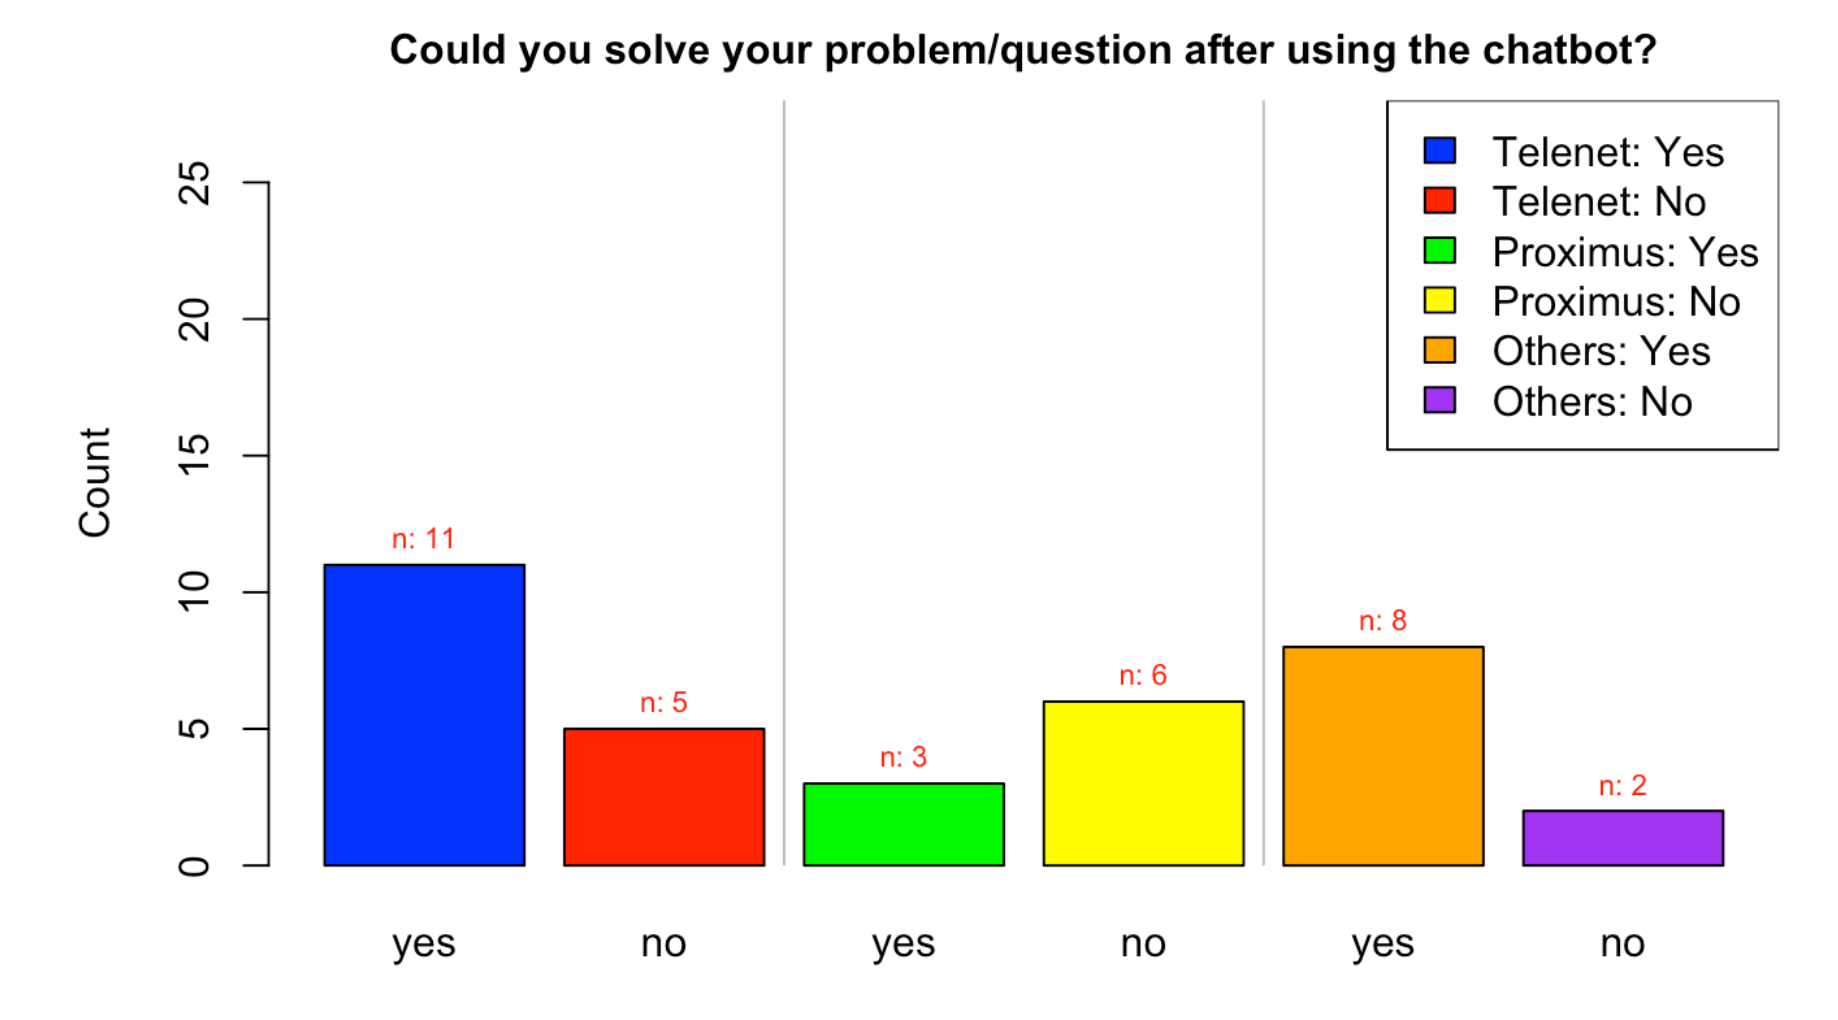
\includegraphics[width=375pt]{../LaTeX/Figures/Comparative/DQ1c.png}
	\caption{Responses about the functional question for \acrshort{qa} 1, question 4.}\label{fig:DQ1c}
\end{figure}
\break
\break
\break
\ul{Attribute 2: Number of services}\\
\break
Attribute 2 looked at the services available and delivered by the chatbot in comparison to a human agent. The responses about whether a chatbot delivers a better service than a human agent were for both Telenet and the others an outstanding no whereas for Proximus, the votes were more divided, almost a 50-50 split (Figure \ref{fig:Q2}).\\
\begin{figure}[!htb]
	\centering
	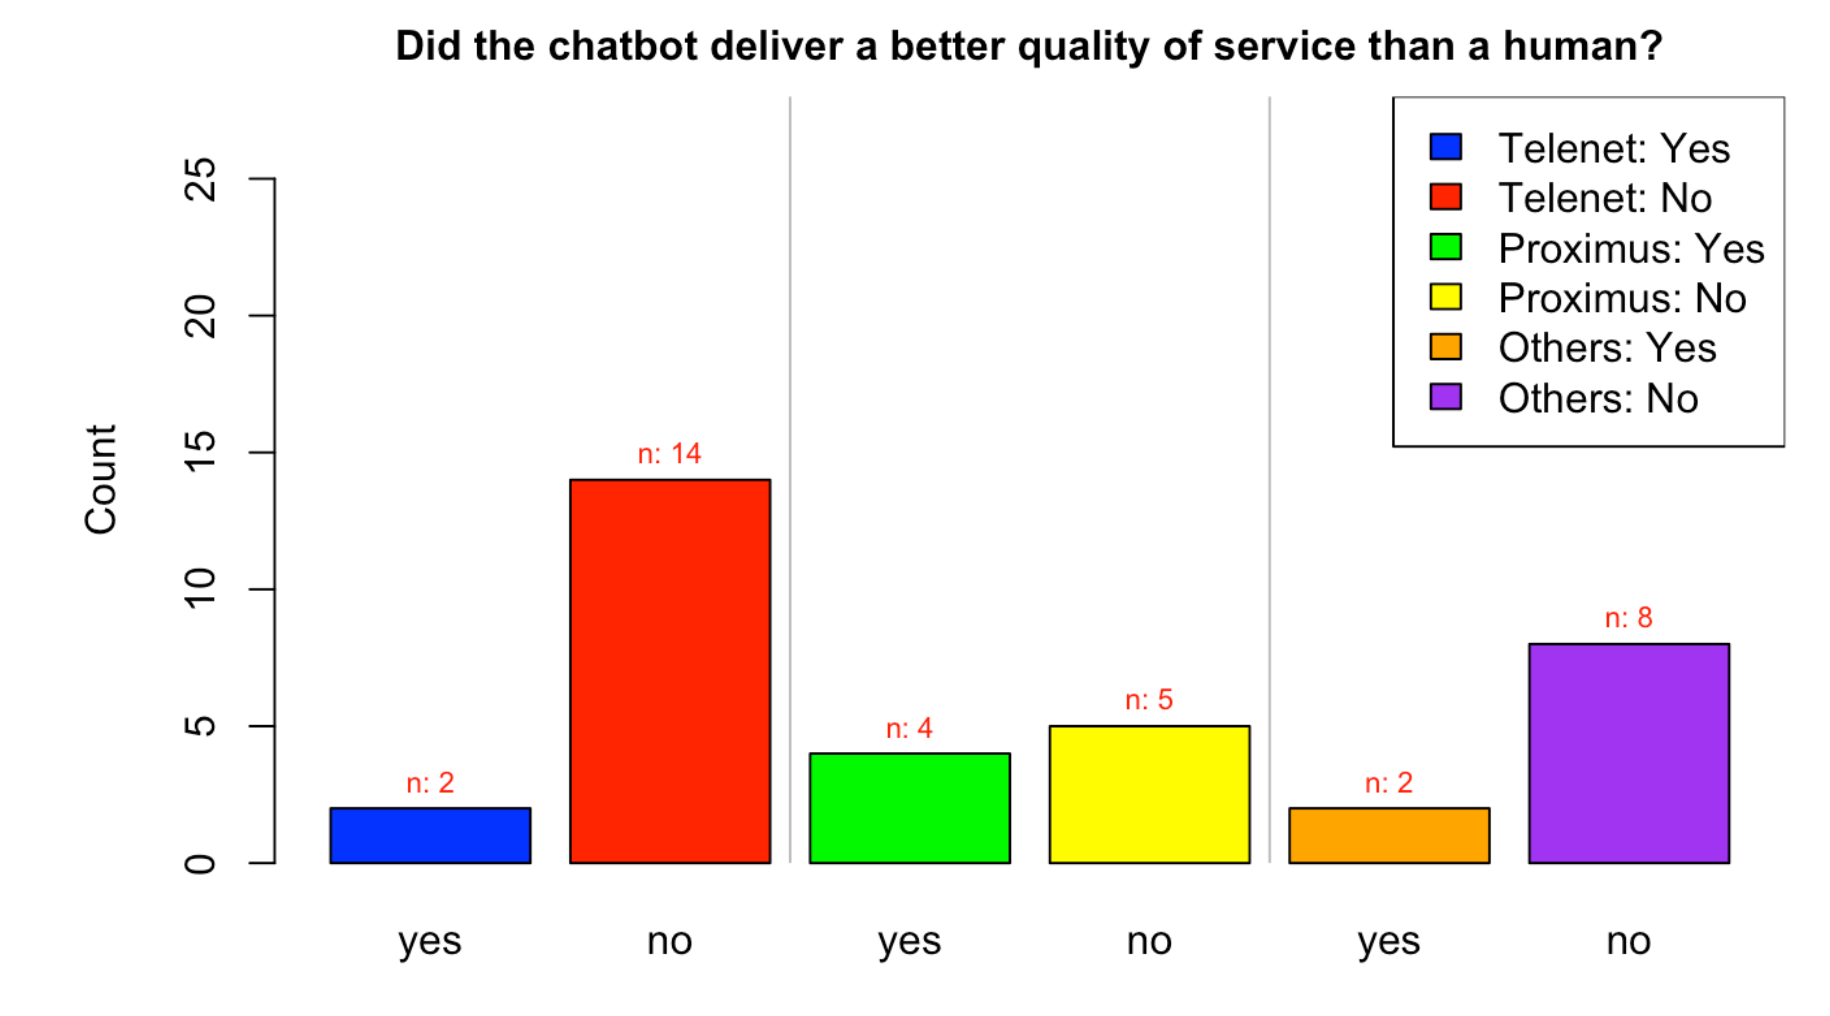
\includegraphics[width=375pt]{../LaTeX/Figures/Comparative/Q2.png}
	\caption{Responses about the functional question for \acrshort{qa} 2.}\label{fig:Q2}
\end{figure}
\break
When asked whether the service delivered by a human was of better quality, the responses for each group were almost always yes (Figure \ref{fig:DQ2}).\\
\begin{figure}[!htb]
	\centering
	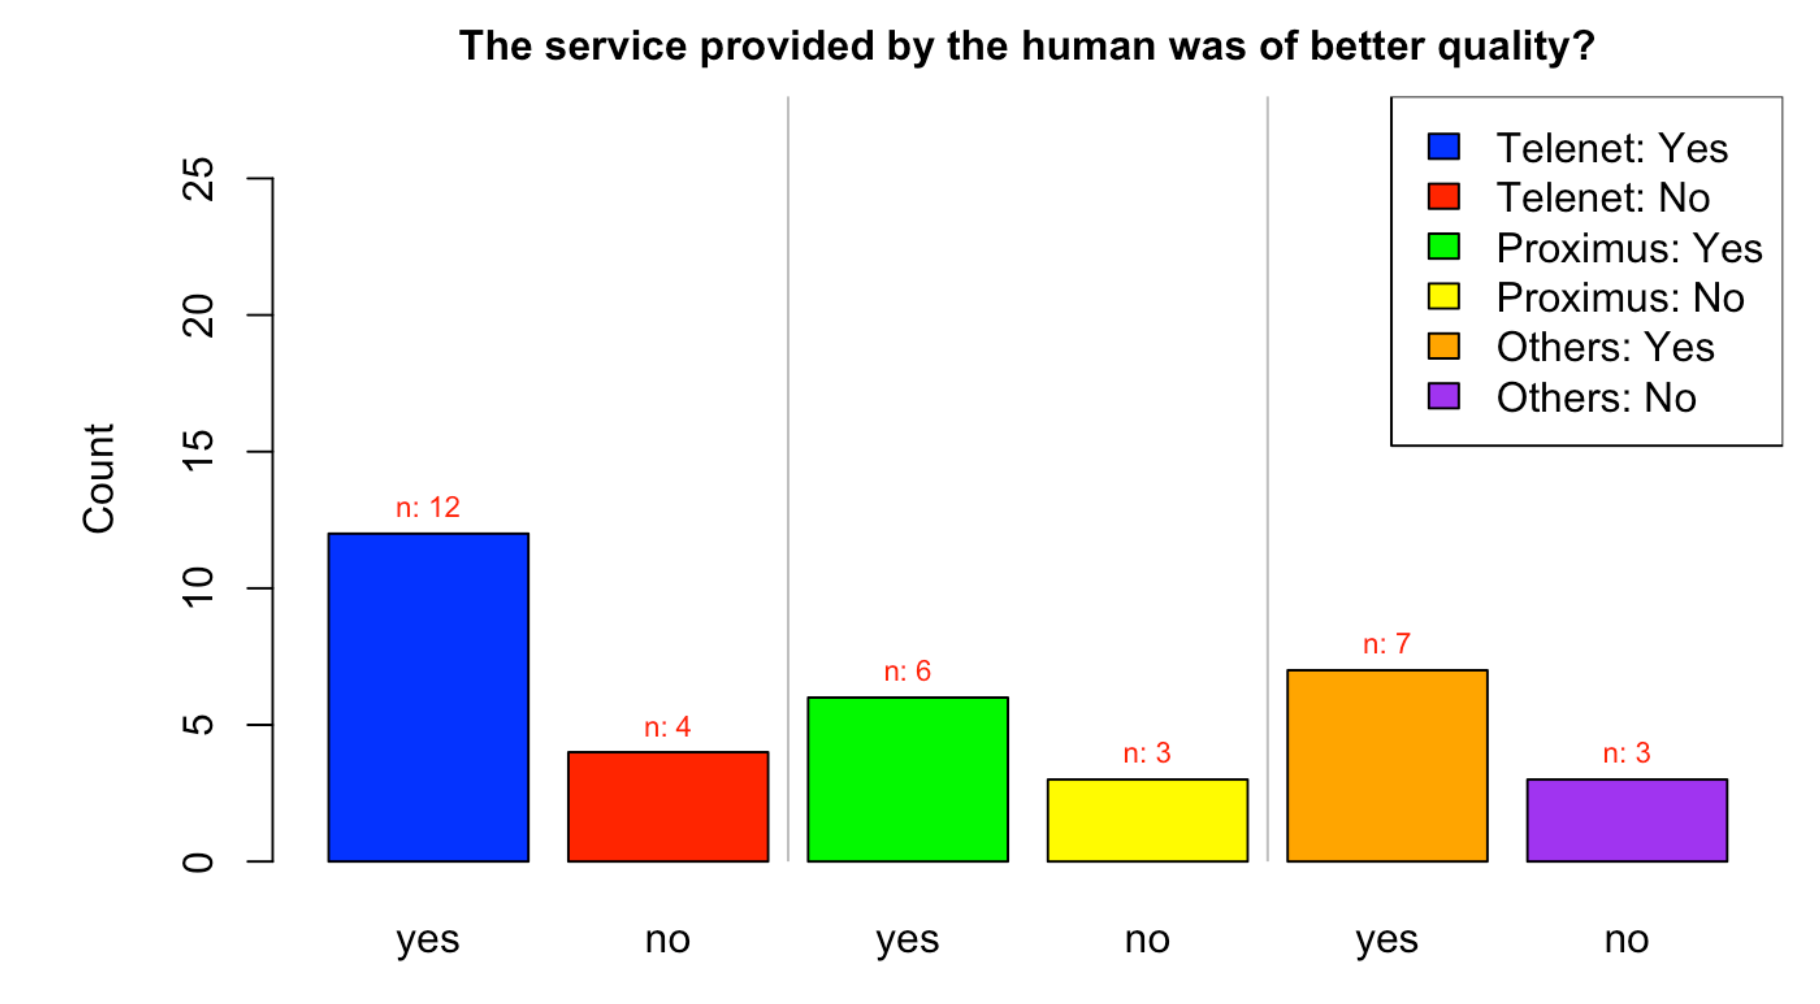
\includegraphics[width=375pt]{../LaTeX/Figures/Comparative/DQ2.png}
	\caption{Responses about the dysfunctional question for \acrshort{qa} 2.}\label{fig:DQ2}
\end{figure}
\break
\ul{Attribute 3: Breadth of knowledge}\\
\break
When presented with the question "Did the chatbot contain enough knowledge to help with your problem", the responses for each group differ a lot. For Telenet, there is a 50-50 split. Proximus on the other hand is mostly negative. This contrasts the others group where the responses were mainly positive (Figure \ref{fig:Q3}).\\
\begin{figure}[!htb]
	\centering
	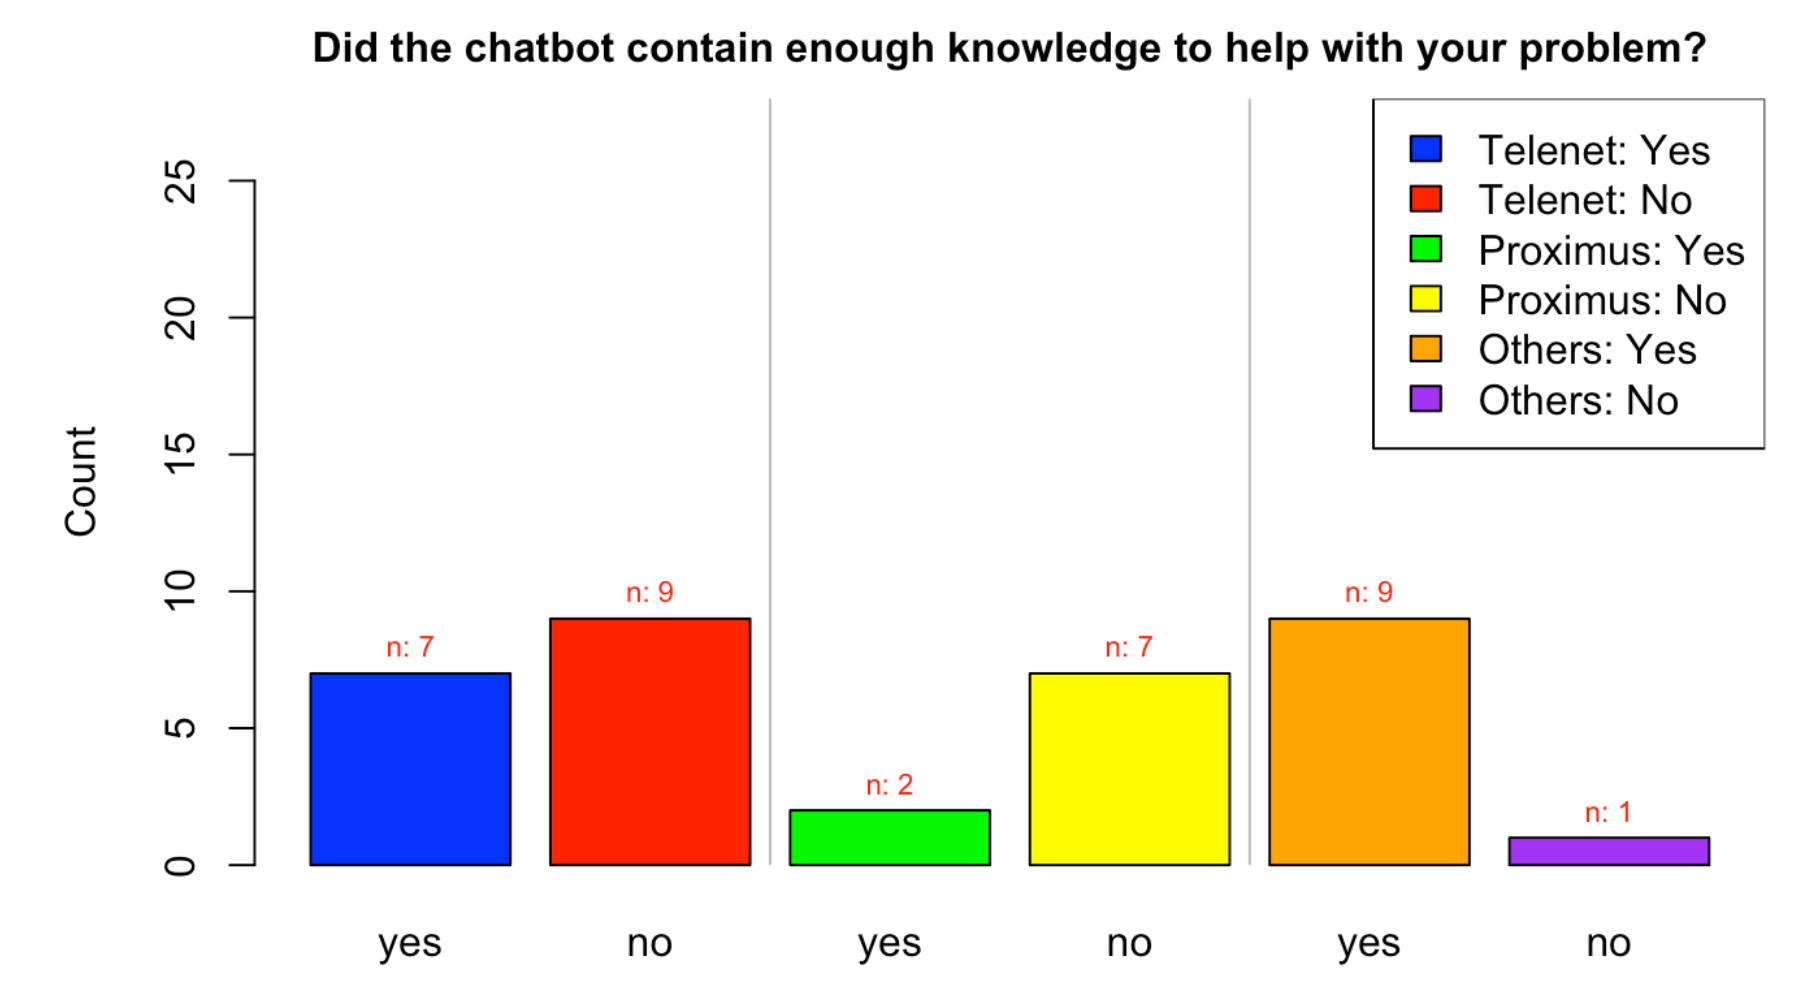
\includegraphics[width=375pt]{../LaTeX/Figures/Comparative/Q3.png}
	\caption{Responses about the functional question for \acrshort{qa} 3, question 1.}\label{fig:Q3}
\end{figure}
\break
When asking the inverse, the answers provided were more streamlined to be mostly negative. In other words, the chatbot knows what he is talking about (Figure \ref{fig:DQ3}).\\
\begin{figure}[!htb]
	\centering
	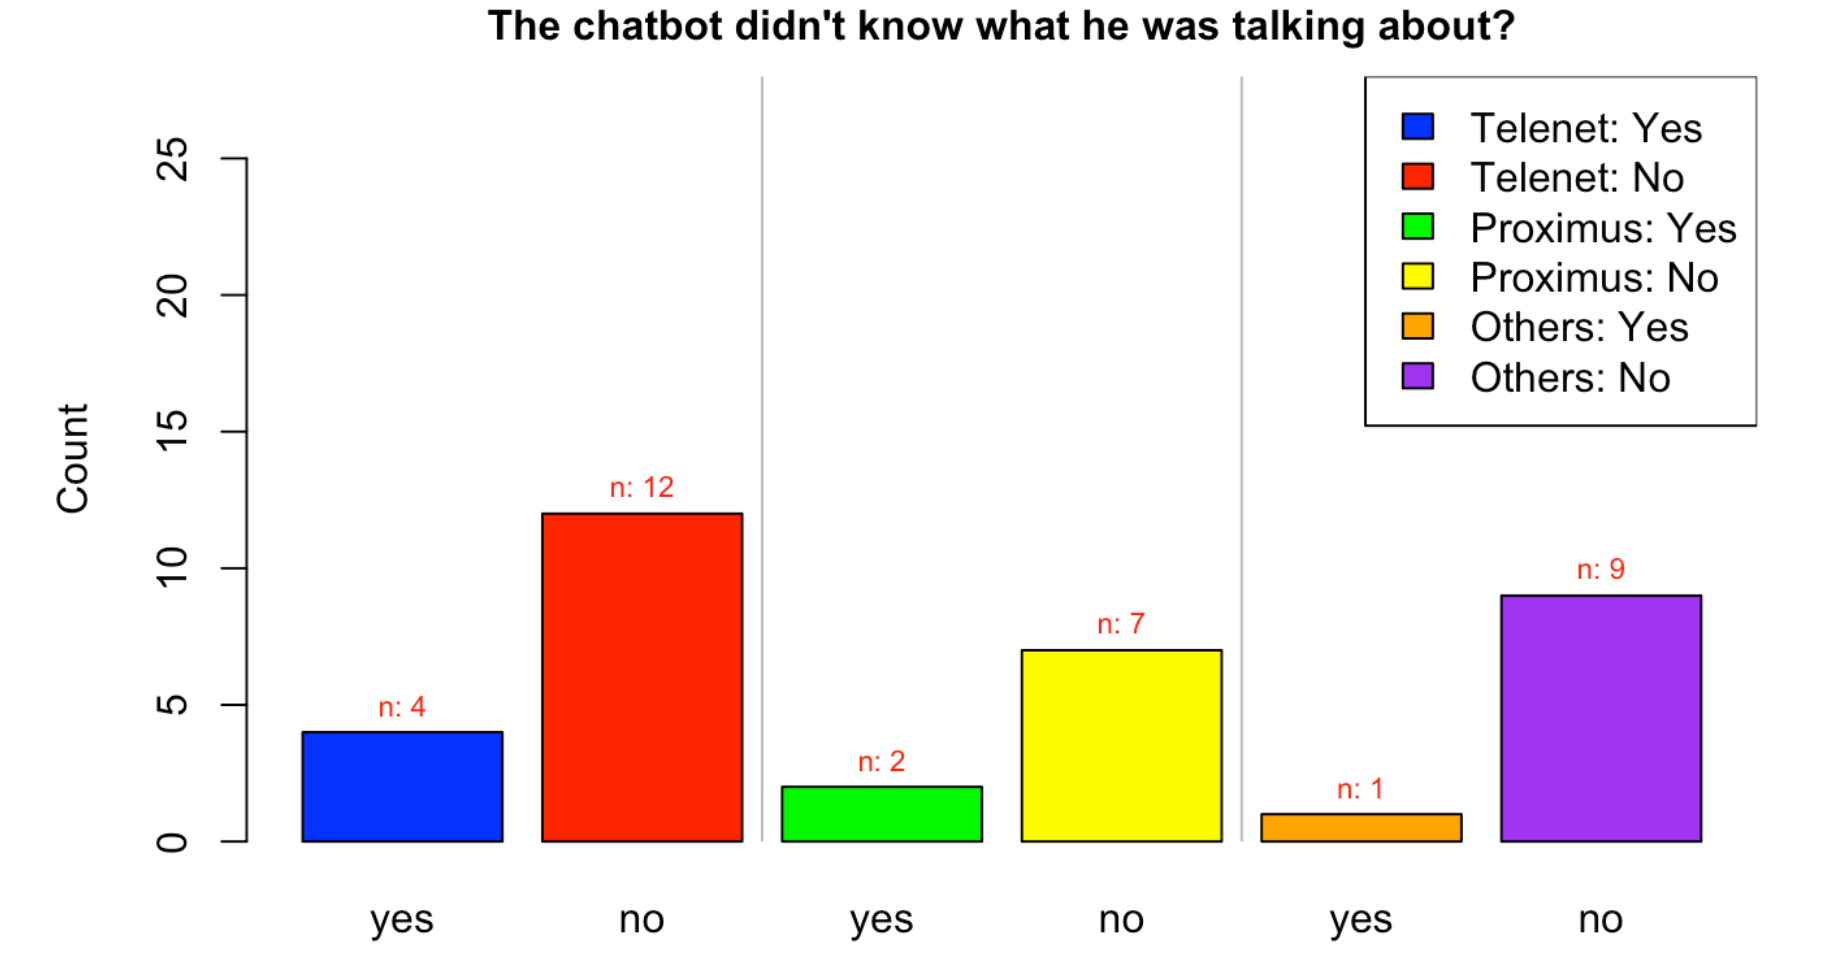
\includegraphics[width=375pt]{../LaTeX/Figures/Comparative/DQ3.png}
	\caption{Responses about the dysfunctional question for \acrshort{qa} 3, question 1.}\label{fig:DQ3}
\end{figure}
\break
The second question checks if the chatbot asked relevant questions to gather extra information about the problem. It measures if the chatbot can gather more information if the given context is not clear enough. Telenet and the others were mostly positive, Proximus has a 50-50 split (Figure \ref{fig:Q3b}).\\
\begin{figure}[!htb]
	\centering
	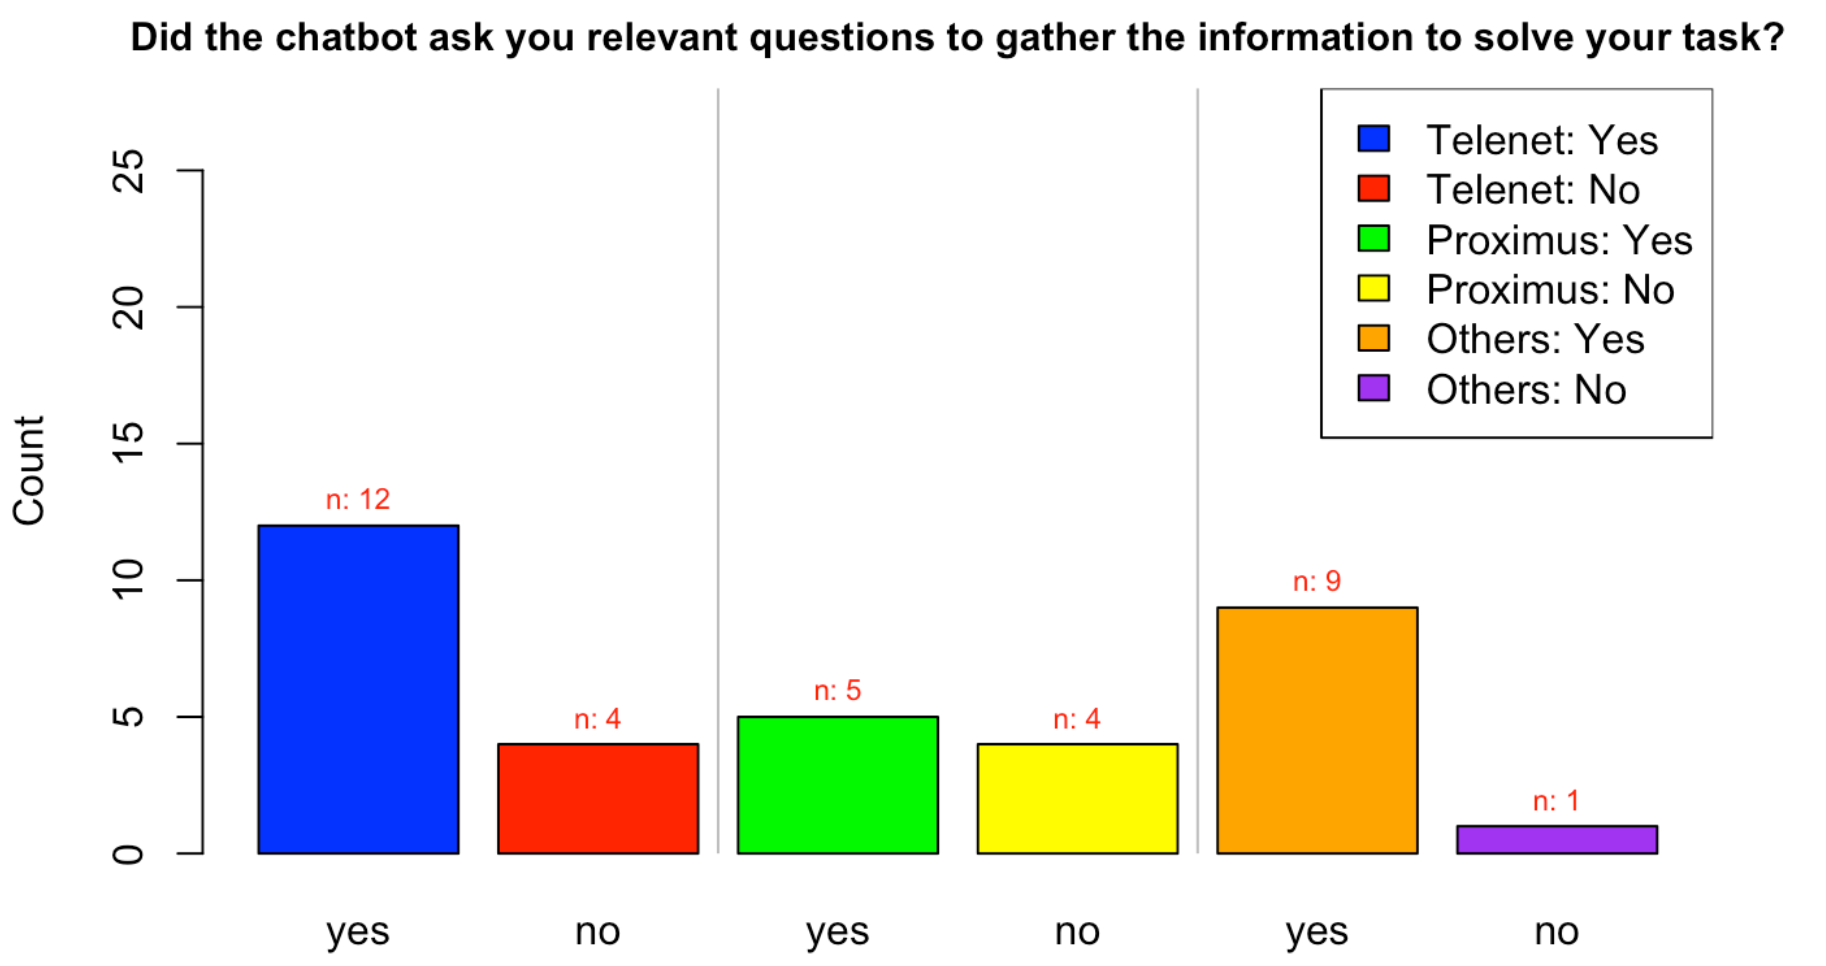
\includegraphics[width=375pt]{../LaTeX/Figures/Comparative/Q3b.png}
	\caption{Responses about the functional question for \acrshort{qa} 3, question 2.}\label{fig:Q3b}
\end{figure}
\break
When looking at the reverse, Telenet seemed to not ask the right questions whereas Proximus and the others were about evenly split (Figure \ref{fig:DQ3b}).\\
\begin{figure}[!htb]
	\centering
	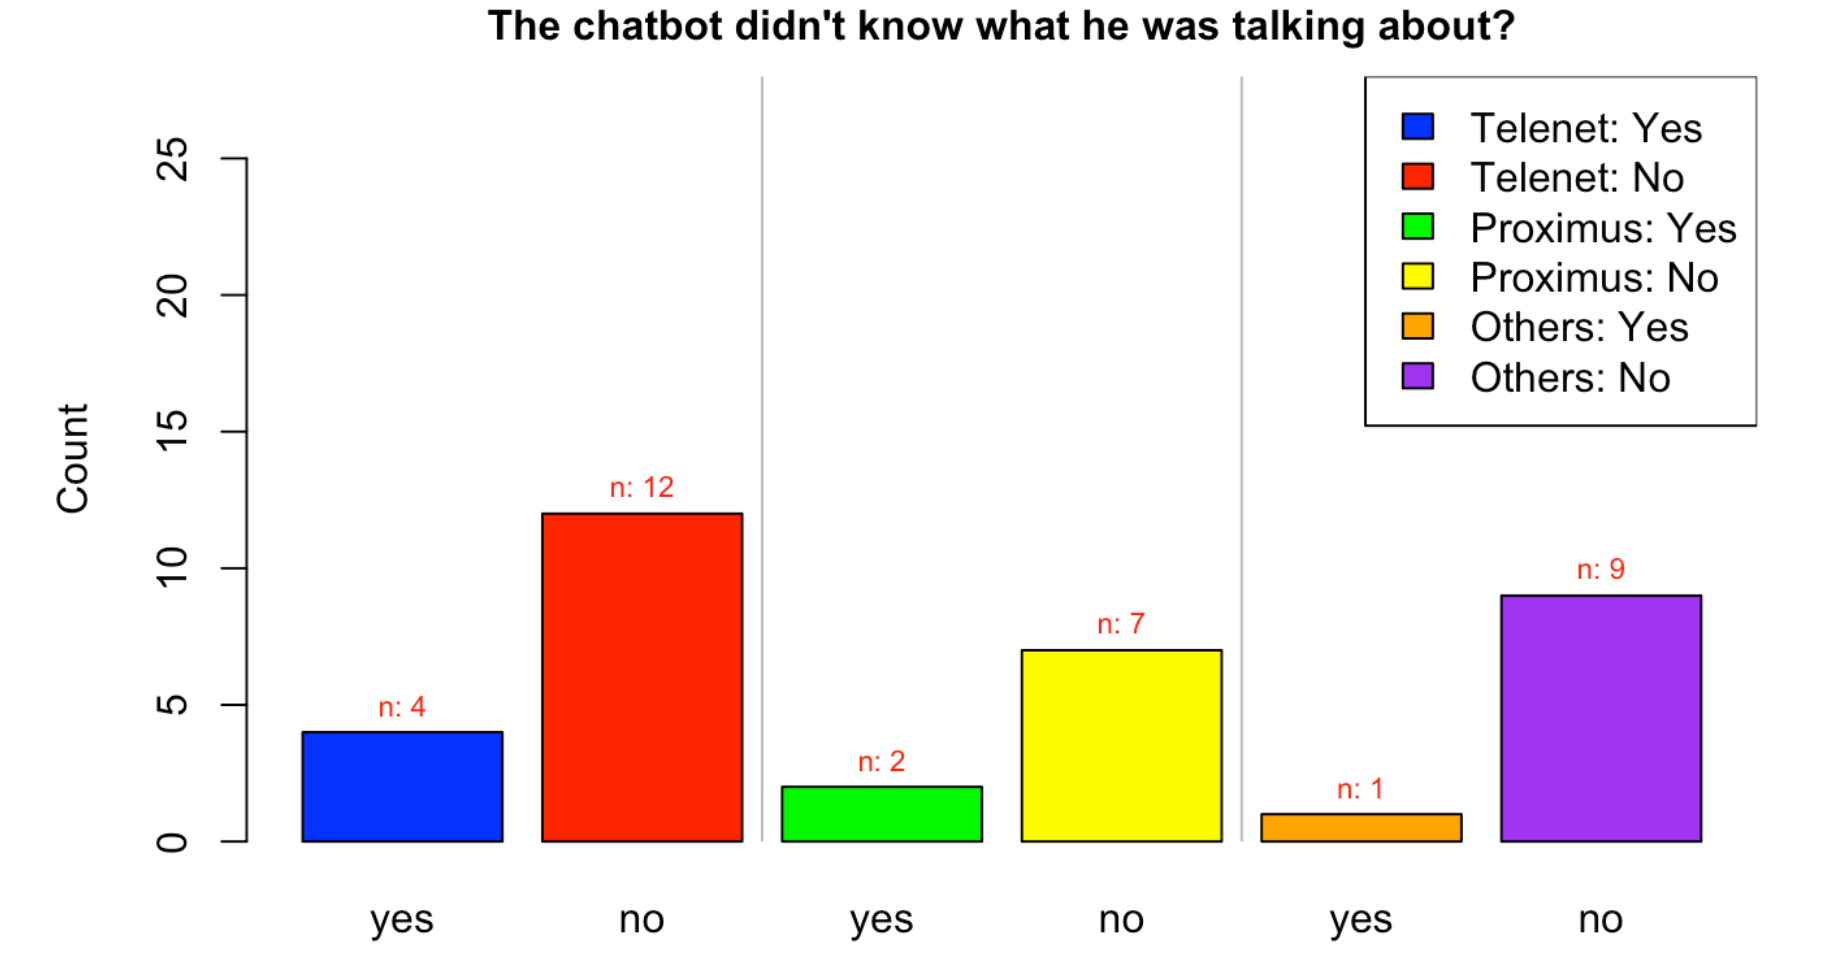
\includegraphics[width=375pt]{../LaTeX/Figures/Comparative/DQ3.png}
	\caption{Responses about the dysfunctional question for \acrshort{qa} 3, question 2.}\label{fig:DQ3b}
\end{figure}
\break 
\break
\break
\break
\break
\ul{Attribute 4: Ease of use}\\
\break
There were not any complications when using any of the chatbots (Figure \ref{fig:Q4}).
\begin{figure}[!htb]
	\centering
	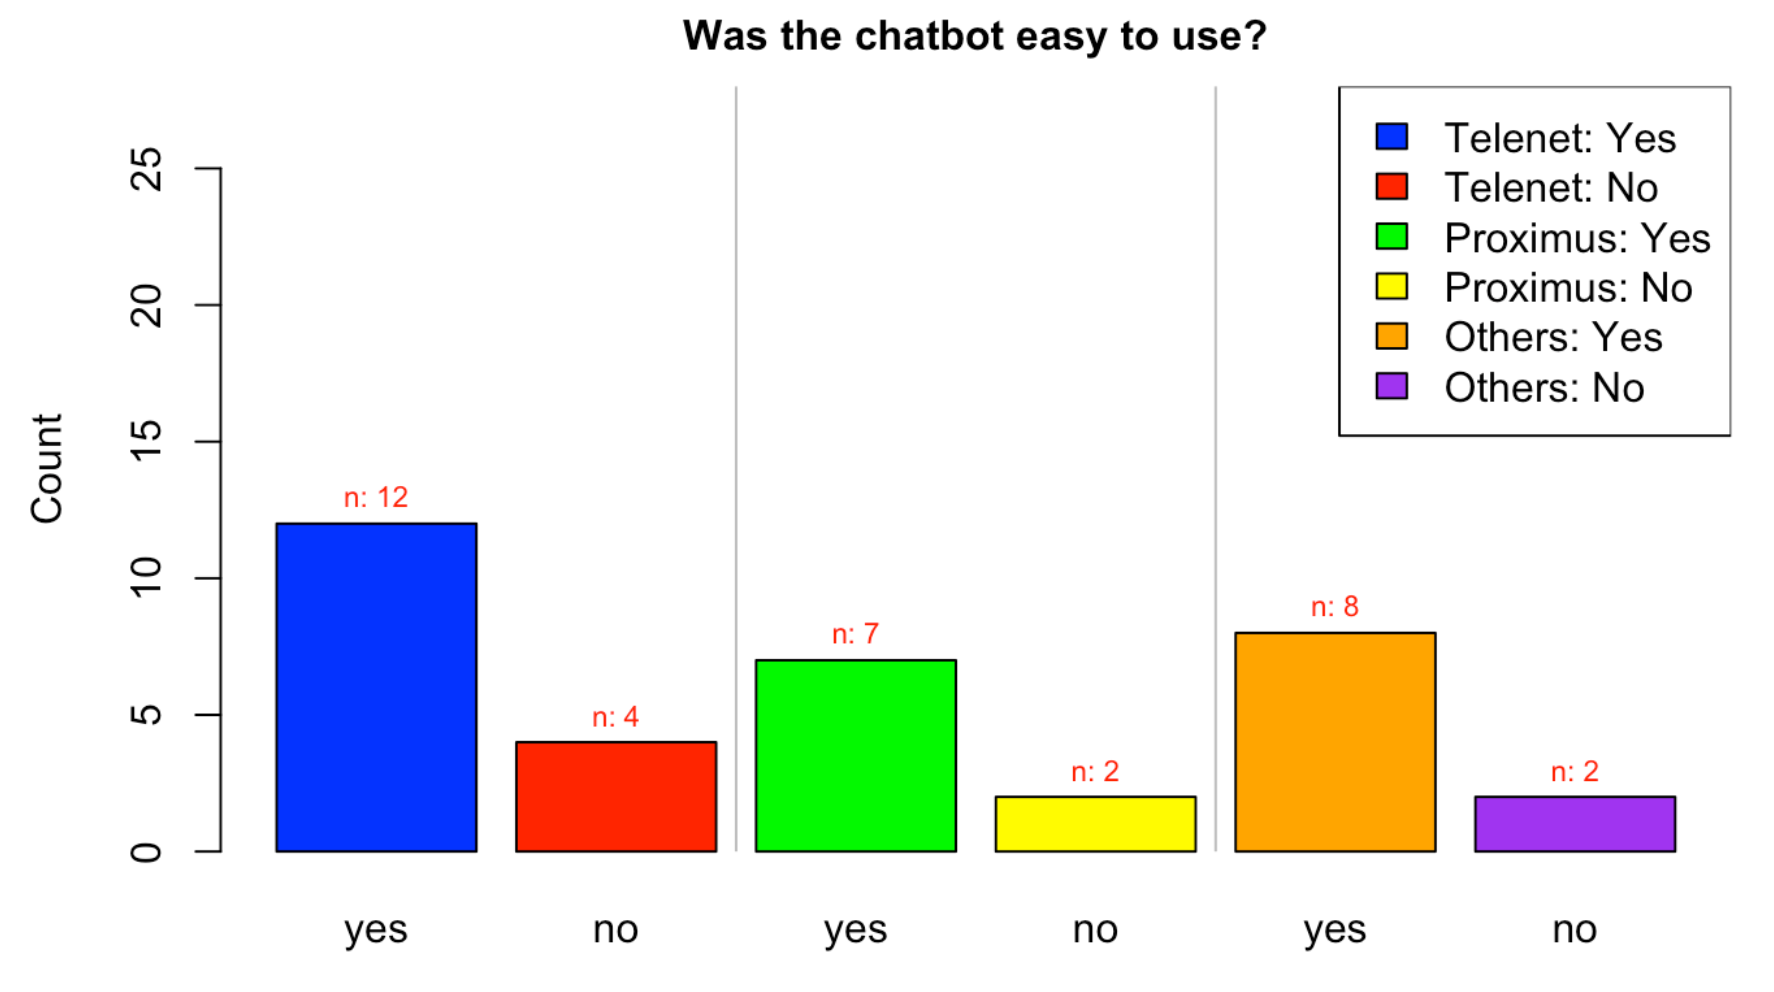
\includegraphics[width=375pt]{../LaTeX/Figures/Comparative/Q4.png}
	\caption{Responses about the functional question for \acrshort{qa} 4.}\label{fig:Q4}
\end{figure}
\break
Looking at the dysfunctional version of this question, the values confirm what has been seen for Telenet and the others but dispute the result for Proximus. There seem to be some problems when using the Proximus chatbot (Figure \ref{fig:DQ4}).\\
\begin{figure}[!htb]
	\centering
	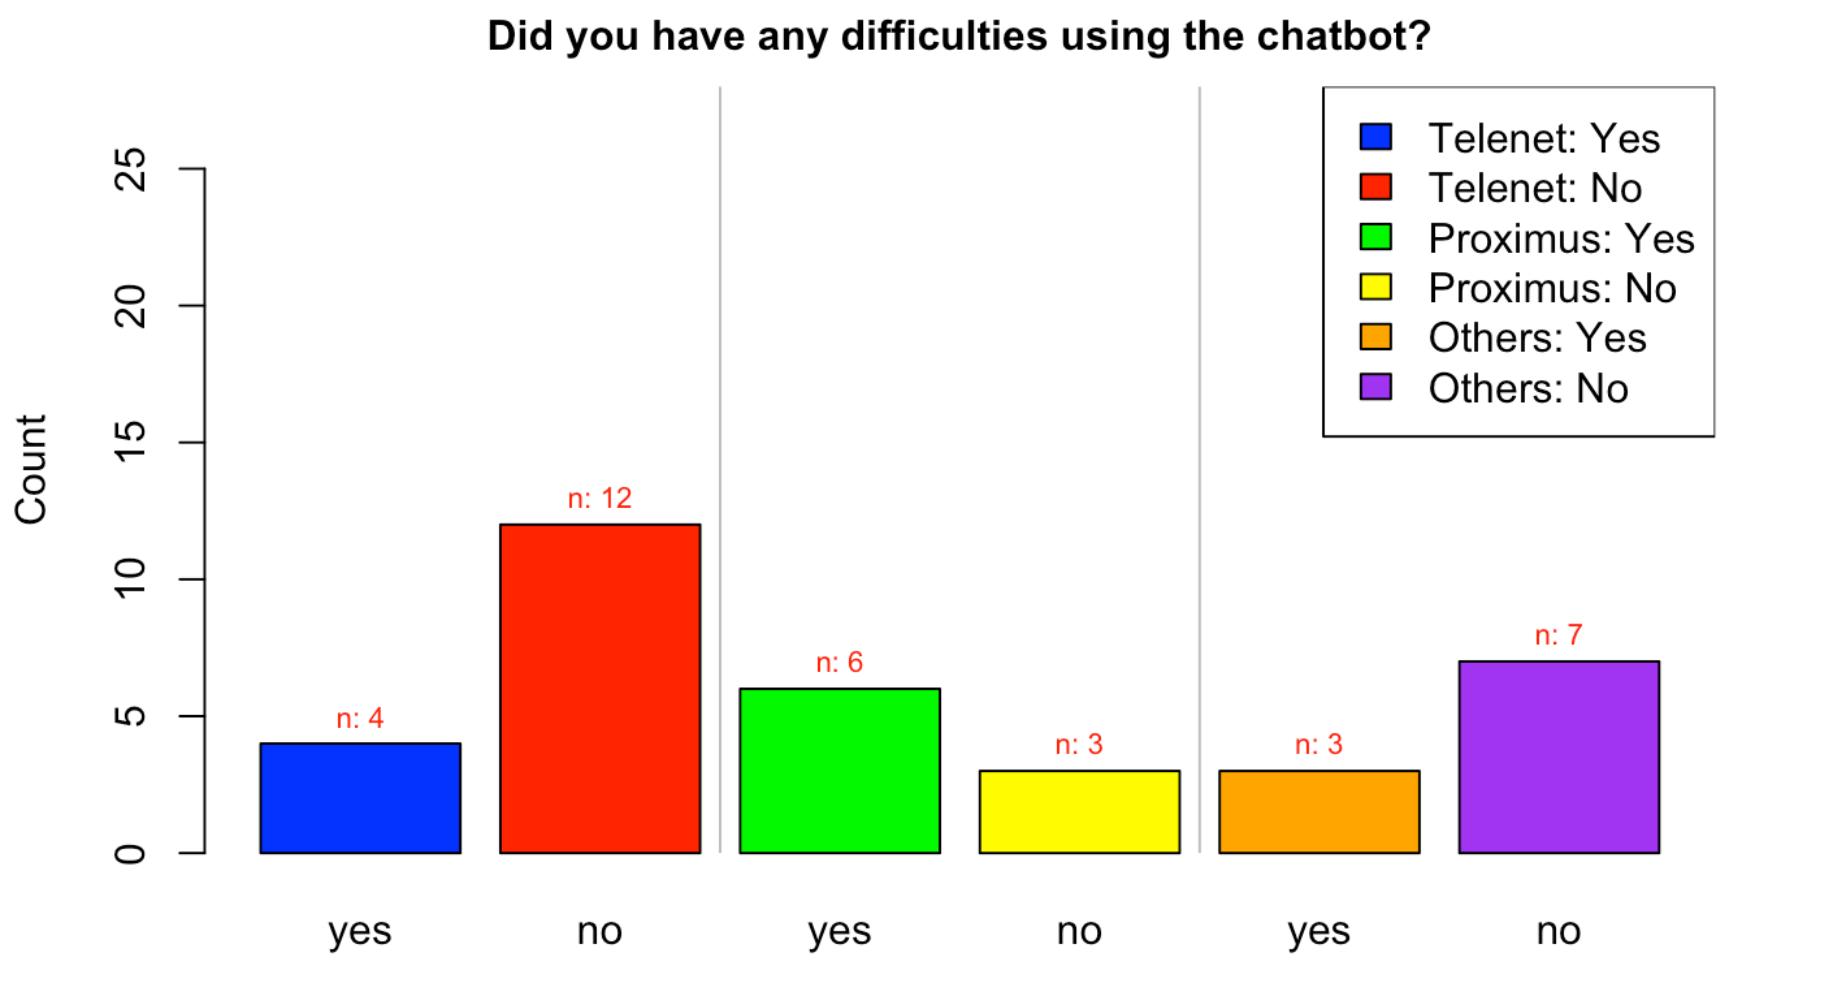
\includegraphics[width=375pt]{../LaTeX/Figures/Comparative/DQ4.png}
	\caption{Responses about the dysfunctional question for \acrshort{qa} 4.}\label{fig:DQ4}
\end{figure}
\break
\ul{Attribute 5: Enjoyable interaction}\\
\break
The fifth attribute takes into consideration the interaction a user has with the chatbot. The first question asked if the chatbot was polite. The data shows that every group generally has a polite chatbot (Figure \ref{fig:Q5}).\\
\begin{figure}[!htb]
	\centering
	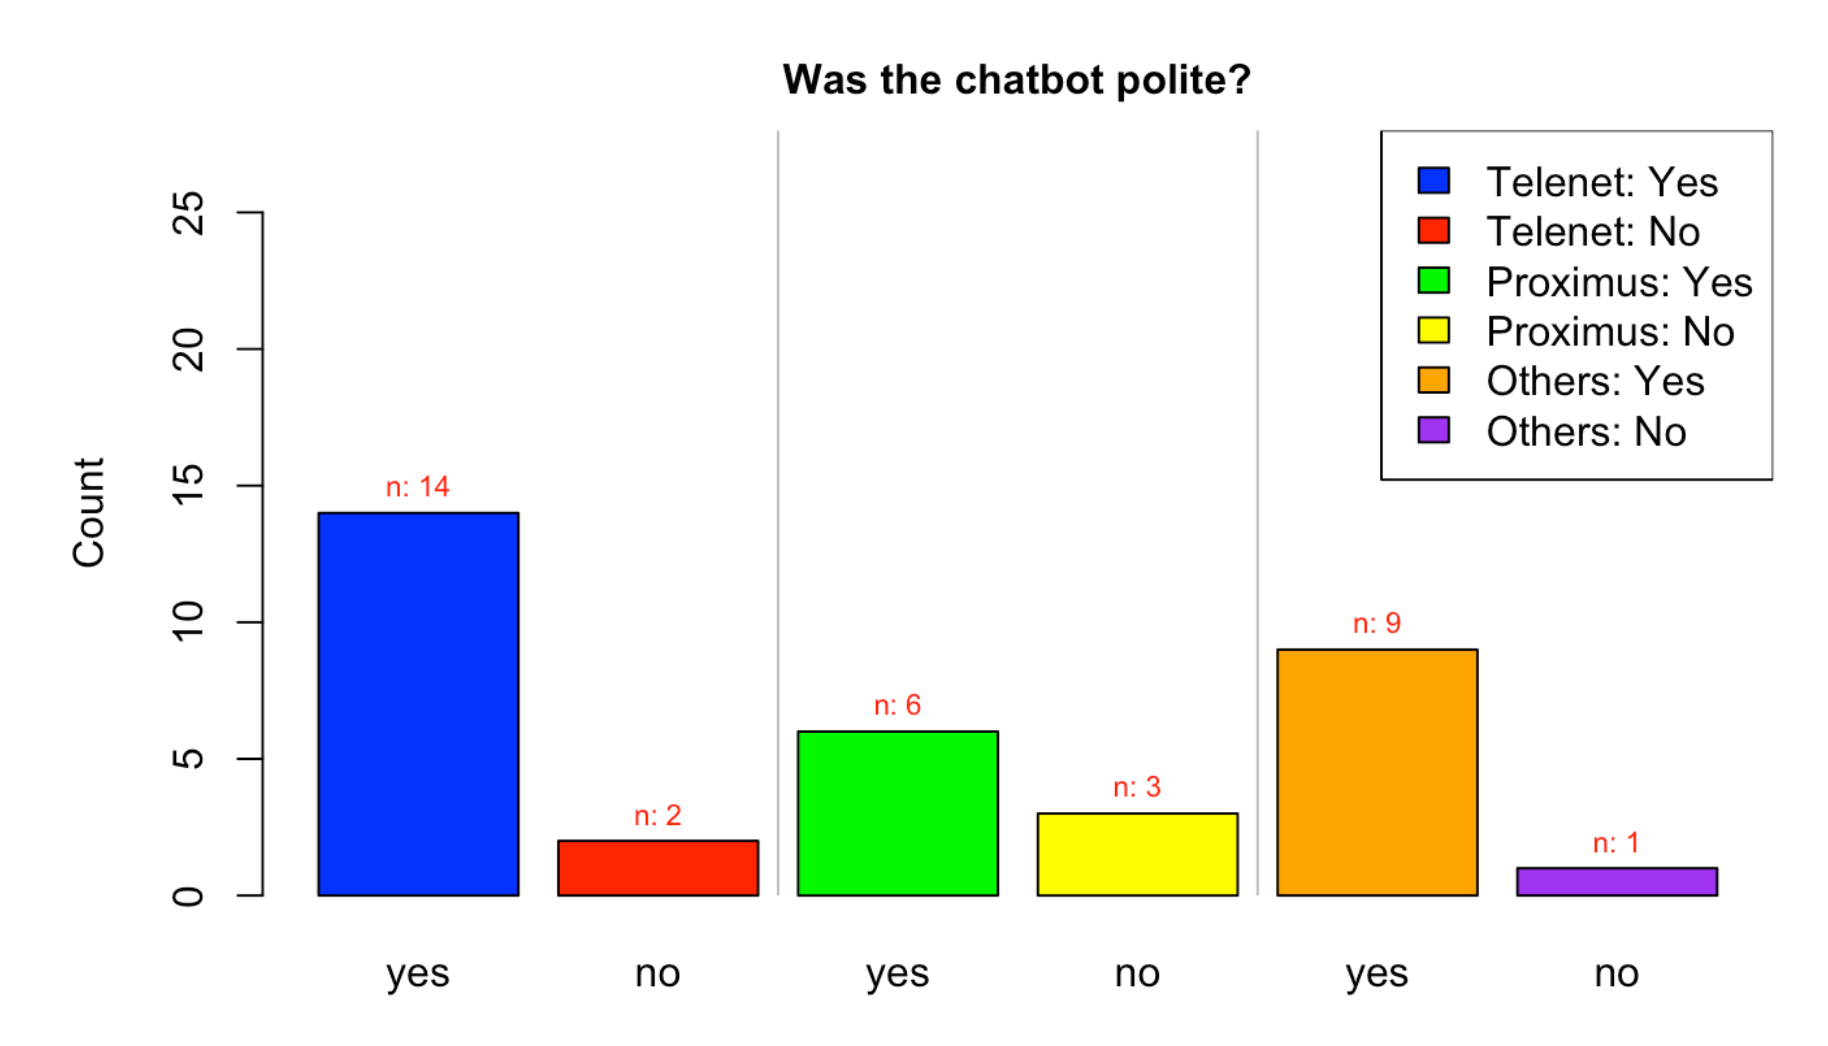
\includegraphics[width=375pt]{../LaTeX/Figures/Comparative/Q5.png}
	\caption{Responses about the functional question for \acrshort{qa} 5, question 1.}\label{fig:Q5}
\end{figure}
When asked if the chatbot interacted in a respectful way, the answers for Telenet were mostly positive, Proximus is once again divided around the 50\% mark and the others scored 100\% (Figure \ref{fig:DQ5}).\\
\begin{figure}[!htb]
	\centering
	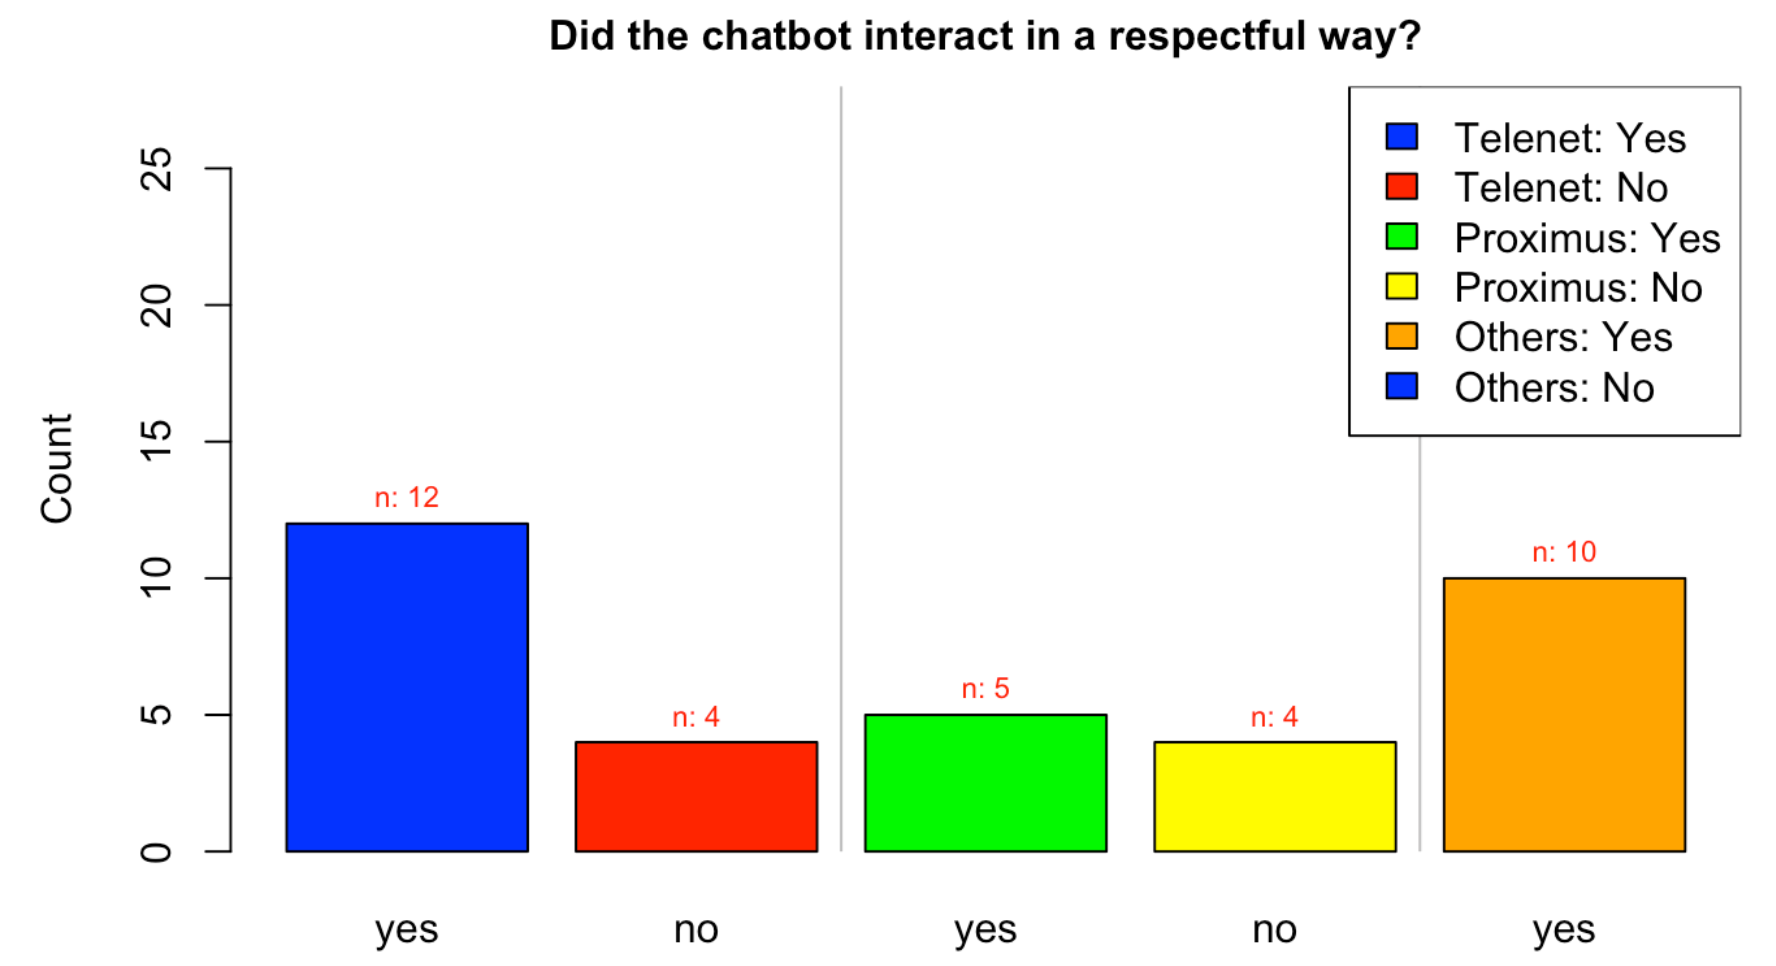
\includegraphics[width=375pt]{../LaTeX/Figures/Comparative/DQ5.png}
	\caption{Responses about the dysfunctional question for \acrshort{qa} 5, question 1.}\label{fig:DQ5}
\end{figure}
\break
The second question asks if the user liked interacting with the chatbot. Telenet is evenly split and both Proximus and the others are mostly positive (Figure \ref{fig:Q5b}).\\
\begin{figure}[!htb]
	\centering
	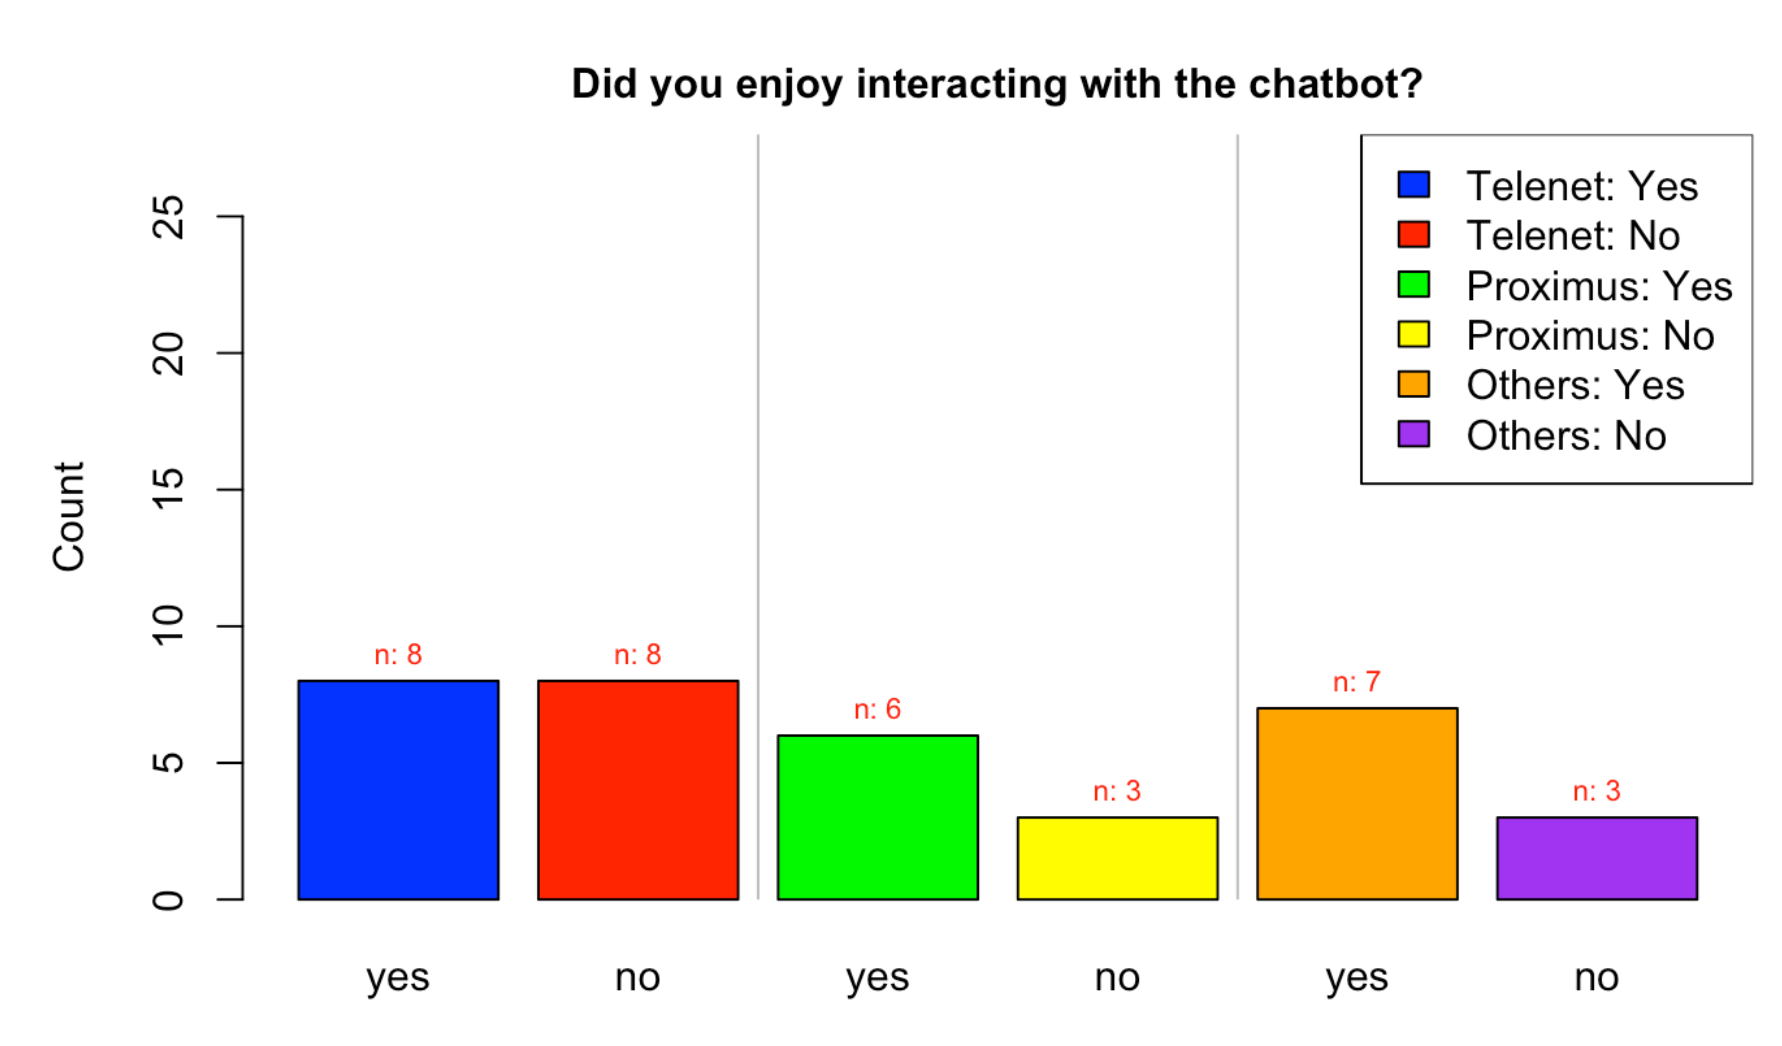
\includegraphics[width=375pt]{../LaTeX/Figures/Comparative/Q5b.png}
	\caption{Responses about the functional question for \acrshort{qa} 5, question 2.}\label{fig:Q5b}
\end{figure}
When asked the reverse, both Telenet and the others are divided evenly. Proximus has more negative than positive responses meaning, it wasn't a task to interact with their chatbot (Figure \ref{fig:DQ5b}).\\
\begin{figure}[!htb]
	\centering
	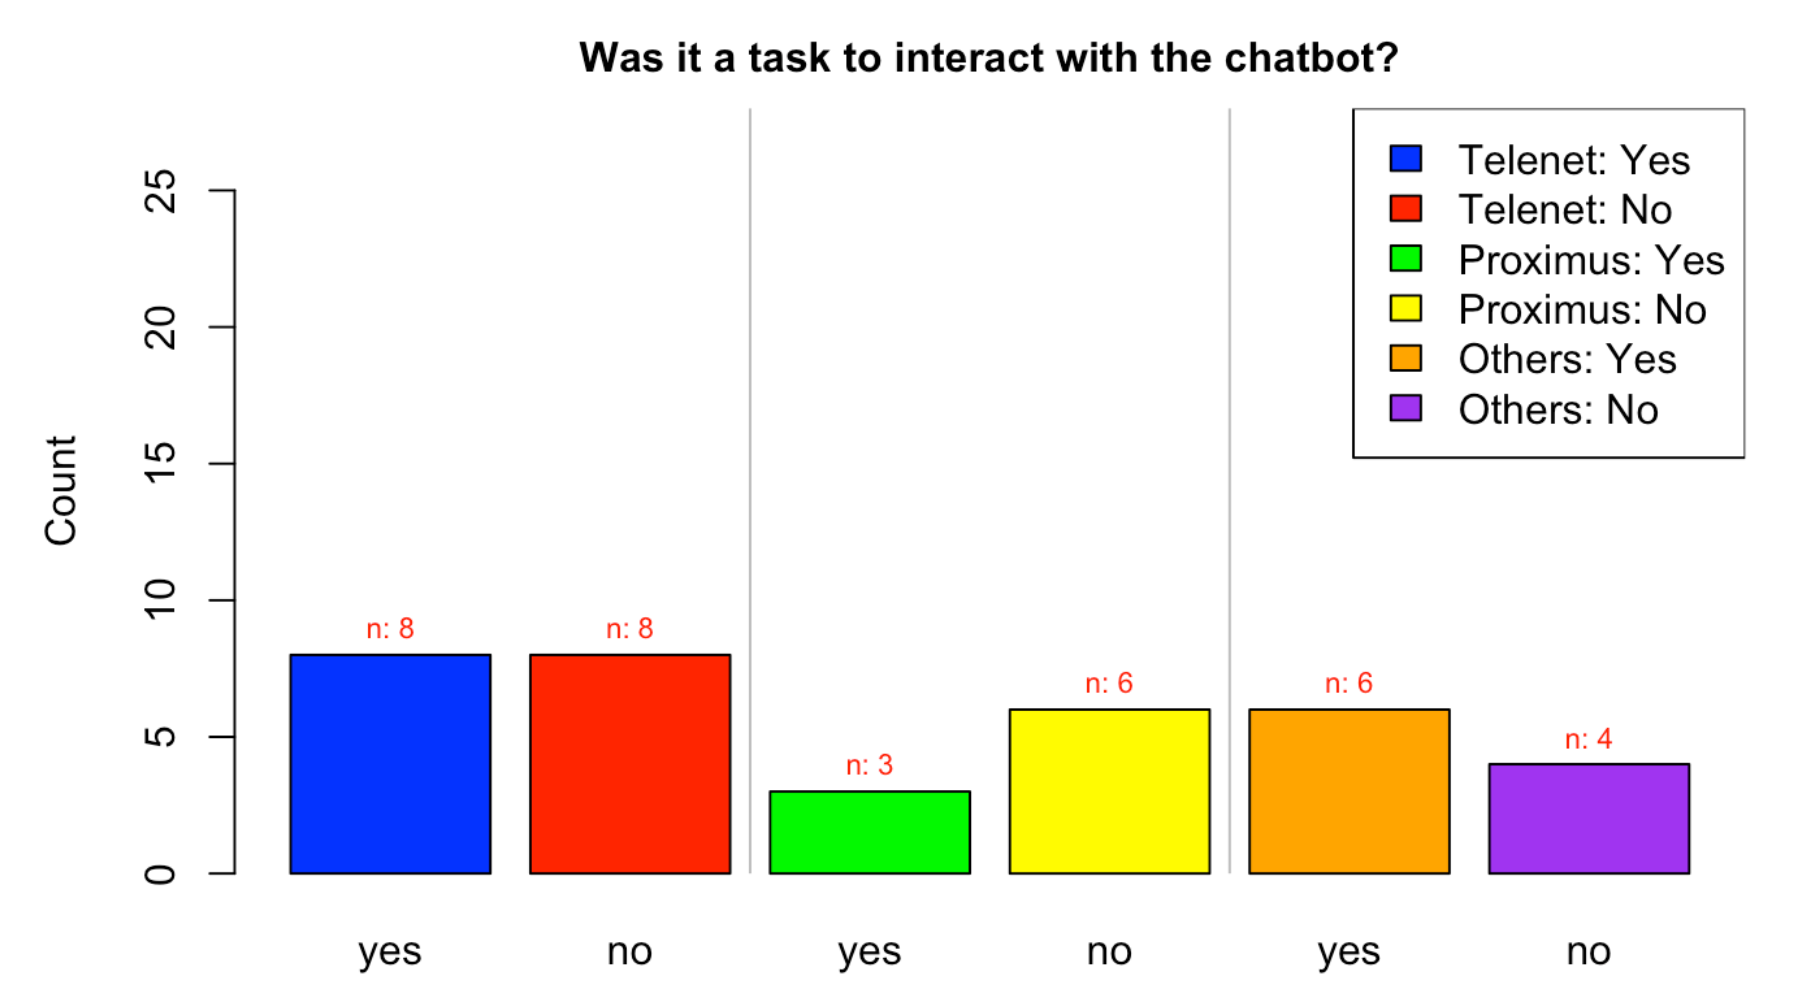
\includegraphics[width=375pt]{../LaTeX/Figures/Comparative/DQ5b.png}
	\caption{Responses about the dysfunctional question for \acrshort{qa} 5, question 2.}\label{fig:DQ5b}
\end{figure}
\FloatBarrier
\FloatBarrier
\subsection{Importance Study - Kano}
\subsubsection{Discrete analysis}
To start with the KANO analysis, there first had to be made a clear mapping between the functional and dysfunctional question and which label of KANO would be assigned to the outcome of this mapping (see Figure \ref{fig:kanoOverview}).
\begin{figure}[htb!]
	\centering
	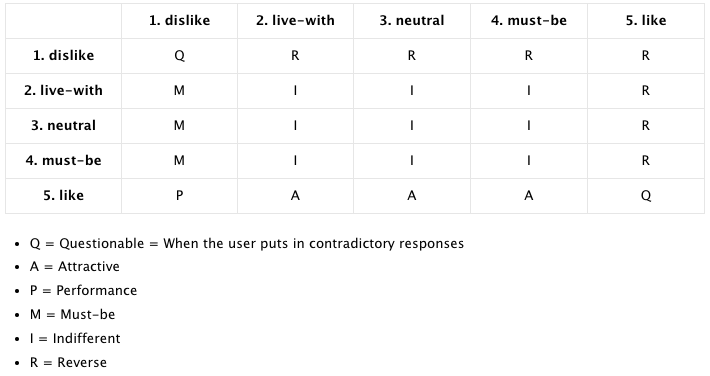
\includegraphics[width=\linewidth]{../LaTeX/Figures/Kano/KANOOverview.png}
	\caption{The mapping between the functional and dysfunctional question and the KANO label associated.}
	\label{fig:kanoOverview}
\end{figure}
\break
Afterwards, for each scenario (section 3.3.3) as well as the general questions of the survey, the answers were counted and added per label. The highest label was assigned. If there was an overlap between two or more labels, the label with the most impact was chosen (see 3.3.2 - Data Evaluation Method).\\
An overview of the label assigned to each entry can be found in Figure \ref{fig:kanoTable}. S1, S2 and S3 refer to the 3 different scenarios.
\begin{figure}[!htb]
	\centering
	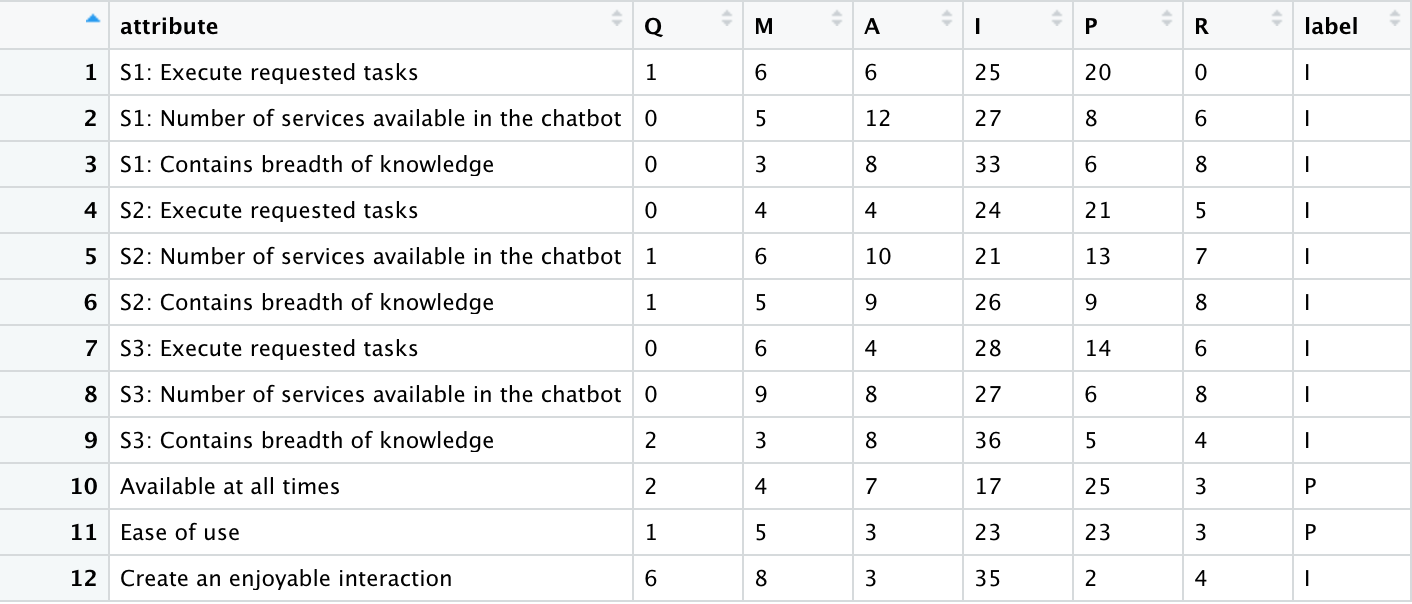
\includegraphics[width=\linewidth]{../LaTeX/Figures/Kano/KanoTable.png}
	\caption{Each entry with it's assigned KANO label.}
	\label{fig:kanoTable}
\end{figure}
\subsubsection{Continuous analysis}
Now, each entry has a label assigned to it and for every entry, the different categories are counted. Based on this, both the satisfaction as well as the dissatisfaction coefficient can be calculated. The calculations can be seen in Figure \ref{fig:satisfactionCoef} and Figure \ref{fig:dissatisfactionCoef}.
\begin{figure}[!htb]
	\centering
	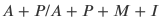
\includegraphics[width=120pt]{../LaTeX/Figures/Kano/SatisfactionCoef.png}
	\caption{The satisfaction coefficient.}
	\label{fig:satisfactionCoef}
\end{figure}
\begin{figure}[!htb]
	\centering
	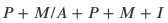
\includegraphics[width=120pt]{../LaTeX/Figures/Kano/DissatisfactionCoef.png}
	\caption{The dissatisfaction coefficient.}
	\label{fig:dissatisfactionCoef}
\end{figure}
\break
After calculating both these scores for each entry, they were plotted in  a scatter plot, dividing them up into one of the four main categories of KANO. The categorisation can be found in Figure \ref{fig:satisfactionPlot}
\begin{figure}[!htb]
	\centering
	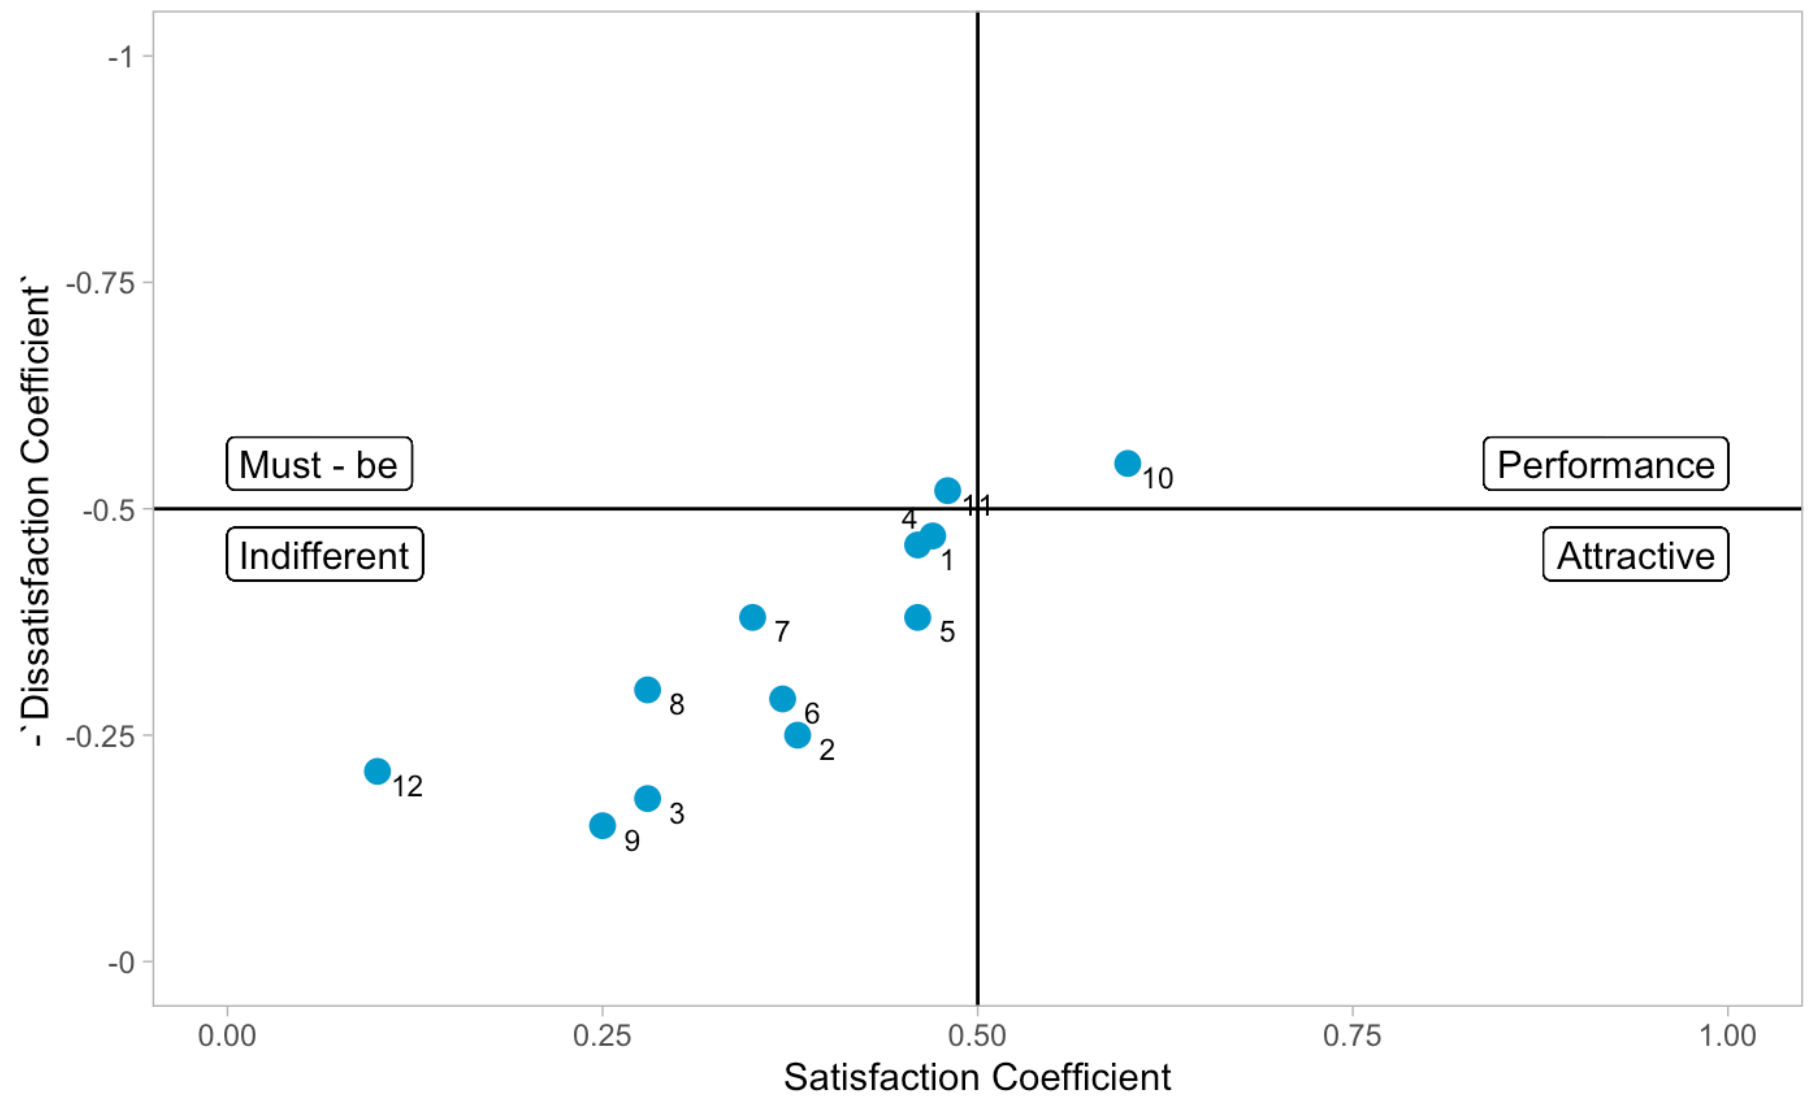
\includegraphics[width=375pt]{../LaTeX/Figures/Kano/SatisfactionPlot.png}
	\caption{The satisfaction/dissatisfaction plot.}
	\label{fig:satisfactionPlot}
\end{figure}

\begin{longtable}{|c|l|}
	\hline
	\textbf{Item} & \multicolumn{1}{c|}{\textbf{Attribute}}         \\ \hline
	\endfirsthead
	\endhead
	\textbf{1}    & S1: Execute requested tasks                     \\ \hline
	\textbf{2}    & S1: Number of services available in the chatbot \\ \hline
	\textbf{3}    & S1: Contains breadth of knowledge               \\ \hline
	\textbf{4}    & S2: Execute requested tasks                     \\ \hline
	\textbf{5}    & S2: Number of services available in the chatbot \\ \hline
	\textbf{6}    & S2: Contains breadth of knowledge               \\ \hline
	\textbf{7}    & S3: Execute requested tasks                     \\ \hline
	\textbf{8}    & S3: Number of services available in the chatbot \\ \hline
	\textbf{9}    & S3: Contains breadth of knowledge               \\ \hline
	\textbf{10}   & Available at all times                          \\ \hline
	\textbf{11}   & Ease of use                                     \\ \hline
	\textbf{12}   & Create an enjoyable interaction                 \\ \hline
	\caption{An Overview of the plotted entries in the satisfaction/dissatisfaction plot.}
	\label{tab:kanoSatisfactionDissatisfactionTable}
\end{longtable}
\FloatBarrier
\FloatBarrier
\section{Discussion}
\subsubsection{RQ1: Are current chatbots effective in helping people and
	solving their problems?}
\ul{H1: Current chatbots execute requested tasks correctly.}\\
At this point, there seems to be a split customer base about the delivered service by the chatbot. Some are happy with the execution of their task where others were not. They also indicate that the chatbot needs help from an agent but this seemed to match their expectations. In the end, most could solve their problem with the help of the chatbot.\\
\break
\ul{H2: Current chatbots can deliver the same services as a human
	agent.}\\
The data clearly shows that people do not think chatbots can deliver the same services as a human agent to the same quality.\\
\break
\ul{H3: Current chatbots contain enough knowledge to provide good
	assistance.}\\
There seems to be a big split between the customers. Depending on the provider, around 50\% think the chatbot is knowledgeable enough to help with their problem. When the chatbot did not have enough context to solve a question, depending on the situation, around 50\% think the chatbot did not ask the right questions to gather the needed information.\\
\break
\textbf{RQ1:} The opinions are divided. In some cases they are effective, in others they are not but they perform up to expectations from the customer.
\subsubsection{RQ2: Are current chatbots easy to use and accessible?}
\ul{H4: Current chatbots are easy to use.}\\
In general, there does not seem to be a problem when using the chatbot.\\
\break
\break
\ul{H5: Current chatbots are available at all times (24/7).}\\
Each provider provides a chatbot that is available 24/7.\\
\break
\textbf{RQ2:} Yes, chatbots are easy to use and accessible.
\subsubsection{RQ3: Do current chatbots create a pleasant customer experience?}
\ul{H6: Current chatbots create an enjoyable interaction.}\\
Chatbots are generally perceived to be polite to interact with and most did not mind interacting with a chatbot.\\
\break
\textbf{RQ3:} It is not yet perceived as enjoyable but it is not a task either.
\subsubsection{Main question}
The influence on the customer experience can be found in the ease of answering simple questions via the chatbot. On the other hand, more complex questions that cannot be solved might lead to frustrations.\\
For the business value, the influence is found in reducing costs for the help desk. The company is 24/7 available for support. The negative aspects force the providers to improve their chatbot with new technologies are more advanced \acrshort{ai} techniques.

\subsection{Quality attributes for telecom chatbots}
\ul{Difference between the scenarios}\\
Looking at the labels assigned to each category in each scenario, it is clear that there is not much difference in importance between the different scenarios. Looking at Figure \ref{fig:satisfactionPlot}, the same attributes for different scenarios are quite close together as well.\\
\break
\ul{General attributes}\\
Ease of use turns out to be a must-be. Compared to the comparative study, this matches the found conclusion and corresponding responses.\\
Availability is a performance attribute. If not/less present, the valued perception of the chatbot would diminish.\\
Customers are indifferent about the experience created by the chatbot. Comparing this to the comparative study, this matches the found answer to RQ3.

\subsection{The future vision of telecom chatbots}
The interviews revealed how chatbots will evolve within the telecom sector and what the most important improvement points are. First and foremost, telecom providers are trying to optimise their services by applying data analysis and fine-tuning algorithms. Additionally, they are looking into sentiment analysis to map out the mood of the customer and to make the bots more language-compatible by means of \acrshort{api}s. As discussed earlier, chatbots are offered on different platforms, one thing  that was discussed several times was harmonising these different platforms so that the chatbot is aware of when the customer is communicating via another platform. In the long term, it can be expected that voice bots will also become more prevalent with possible integrations to smart speakers such as Google home and Alexa.
\FloatBarrier